% CUMCM 2026 B. Class = latexstudio/CUMCMThesis.
\documentclass{cumcmthesis}
\usepackage{unicode-math}
\setmathfont{Cambria Math}
\setmonofont{Courier New}
\setCJKmonofont{FangSong}
\usepackage{amsmath}
\usepackage{graphicx}
\usepackage{booktabs}
\usepackage{longtable}
\usepackage{array}
\usepackage{placeins}
\usepackage{xurl}

\title{无线电干扰源的交会可行集与机器狗清除策略}
\tihao{B}
\baominghao{202617201069}
\schoolname{Operator}
\membera{A}
\memberb{B}
\memberc{C}
\supervisor{—}

\begin{document}
\maketitle

\begin{abstract}
无线电测向把示向度误差限制在正负1度。本文将每条读数解释为半角1度的凸楔形，定位区域取诸楔之交；第二检测点沿第一示向度的正交基线布置；全向源采用9点侦听网和严格覆盖剪枝完成发现，再以距离上界收缩进入光学清除窗；定向源采用边长850 m的三角格网给出闭半平面瓣上的发现证书，听到后进入保扇形追逐。
问题一：合成正交交会例的对径圆覆盖为1；未与场地圆盘相交的两站有界样本覆盖率为1，相交裁剪后覆盖率为0.955；边长80 m的等边三角形对径圆覆盖为0。
问题二：第二检测点取轴上交角不小于45度的覆盖点，轴向距离800 m、横向偏移700 m。网格分位点横向偏移690.90909 m的事后直径中位数为48.2745 m，楔内70个样本上一次清除比例为0.2142857。固定轴向1100 m时，横向200 m的事后直径显著大于横向800 m。
问题三：9点网覆盖半径约956.051 m；有界收缩使每个已发现源最多再用7次动作清除，全任务动作上界为294。48个独立离线模型场景均全清；官方修订版测试尚待完成。
问题四：三角格网共37个侦听点，间距850 m，覆盖半径为490.7477288111819 m，小于500 m；平移量500 m时距离和为990.7477288111819 m。不合格间距上覆盖半径为519.6152422706632 m，不存在合格平移量。光学方格边长25 m的外接半径为17.677669529663685 m，小于20 m。
\keywords{无线电测向，交会定位，凸楔形，Jung定理，三角格网}
\end{abstract}

\section{问题重述}

\subsection{背景}

无线电干扰源的定位与清除是频谱管理中的紧迫任务。传统流程把工作分成初步监测、区域排查和精准定位三个阶段：前两个阶段用固定站、监测车或无人机圈出目标分布区域，最后一公里仍常由技术人员携带便携测向机徒步完成。环境遮挡、低功率辐射和定向波束都会使单点场强判断失效，完成时间又直接决定干扰的残留影响。题目因此提出：在半径1800 m的已知圆域内，用搭载测向机与激光清除装置的机器狗代替人工，建立可执行的自动定位与清除模型。

测向交会并不是新问题。Stansfield早年就把多站示向度的交会写成统计定位，并指出“三角形帽”（cocked hat）的大小本身并不等于定位可靠度\cite{stansfield1947}。无源测向的误差传播随后被系统整理：方位观测是非线性的，几何构型决定可观测性与协方差形状\cite{torrieri1984,foy1976}。单站纯方位跟踪还要求观测平台作侧向机动，否则距离不可辨\cite{nardone1984}。这些经典结论进入本题时必须改写：题目把误差明确限制在$[-1^\circ,1^\circ]$，并且要求输出的是定位区域的直径，而不是一个最大似然点。因此本文把示向度读数解释为楔形可行集的轴，把交会解释为凸集相交，把清除解释为把该凸集送进半径20 m的光学窗口。

\subsection{问题提出}

坐标系以场地圆心为原点，正东为$x$轴正向，正北为$y$轴正向，单位为米。示向度是从$x$轴逆时针转到“检测点指向干扰源”的角度，取值$[0^\circ,360^\circ)$。干扰源个数未知，频道取自$1$至$20$且互不相同、不随时间改变。全向源覆盖$360^\circ$；定向源覆盖其指向两侧各$90^\circ$。有效接收半径落在$[1000,1500]$ m，事先未知。机器狗速度5 m/s，换台1 s，检测5 s，光学精定位3 s，激光清除2 s。光学清除只依赖距离，不依赖波束朝向。同一地点重复检测不改变示向度误差。附件1与附件2给出HTTP接口与测试流程，并不提供问题1的站点坐标表。冻结附件的数据集摘要为\path{sha256:50bf04217eb3e8e7d3ce8b4a84f228b46dcfd93eebae187b443adb7724b2440e}。

四个问题彼此独立，不能并成同一目标函数。

\begin{enumerate}
\item 已知若干检测点及对应示向度，给出交会多边形直径的算法，并判断以该直径为直径的圆能否覆盖定位区域。
\item 已知全向源在一个检测点的示向度，给出第二个检测点的选择策略与候选区域。
\item 场地内10至16个全向源，一只机器狗从原点、频道1出发，自动定位清除；用演练统计检验清除比例与平均时间。
\item 混入未知朝向的定向源，其余条件同问题三，再给出策略并通过演练检验。
\end{enumerate}

题目要求在充分演练之后，按表1的四个字段报告三次正式测试：案例编码、清除干扰源个数、平均定位清除时间、程序运行时间。正式测试占用不可撤回的次数。本文把几何判定、侦听覆盖与演练窗口统计分开书写：演练行只出现在问题三、问题四的演练表中，正式测试表按题目格式列出并留待窗口核验后填入。论文体例遵循竞赛格式规范\cite{format}。

\section{问题分析}

四问对应三类任务：凸可行集的几何度量、第二站的正交基线设计、以及带时间代价的搜索清除。如图\ref{fig:framework}所示，测向读数先变成楔形，楔形相交得到定位区域，区域直径决定一次清除是否充分；第二站把交角抬到接近直角。侦听覆盖必须把距离可听与朝向可听分开：最小有效接收半径只约束距离因子$R_{\mathrm{eff}}$，并不约束波束朝向。在全向假设下，原点加8环的9点网对场地最近距离有闭式上界$\rho\approx 956.05\,\mathrm{m}<1000\,\mathrm{m}$，当场地点到某侦听点的距离不超过该半径时必被听到。定向源即使落在$R_{\mathrm{eff}}$球内，仍可因$180^\circ$瓣的背面而听不到；问题四因此改用边长$850\,\mathrm{m}$的三角格网，把发现写成覆盖半径$\rho=s/\sqrt{3}<500\,\mathrm{m}$的闭式证书，而不是抽样覆盖率。全向源在有限覆盖阶段扫完静默频道后，再按距离上界收缩清除；定向源在格点听到后进入保扇形追逐。四问在几何上依次衔接：全向距离覆盖与有限步清除在问题三证明，定向瓣的发现证书留给问题四。

\begin{figure}[htbp]
\centering
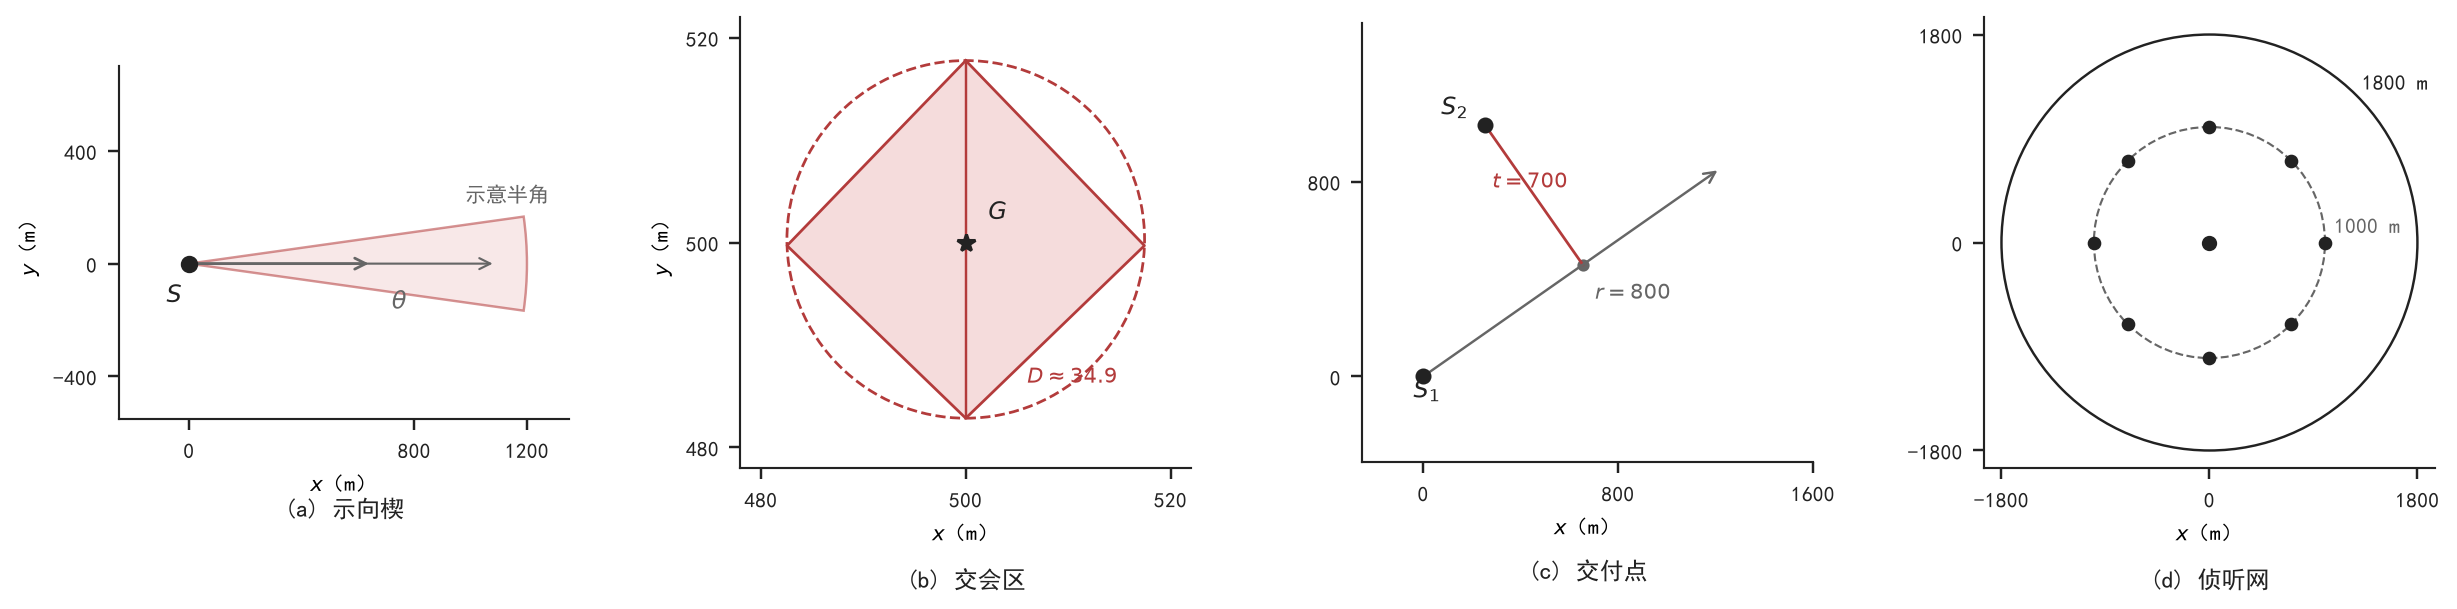
\includegraphics[width=0.98\textwidth]{figures/framework.png}
\caption{四问几何衔接。(a) 示向楔（半角为示意放大，正文取$1^\circ$）；(b) 交会区与对径圆；(c) 交付点$(r,t)=(800,700)$ m，不是网格分位点$|t|=690.9$ m；(d) 侦听网，虚线为1000 m，实线为1800 m。}
\label{fig:framework}
\end{figure}

\subsection{问题一的分析}

交会定位的教科书图像是两条射线交于一点。题目却把误差写成闭区间，并且强调同一地点的误差固定、不同地点才呈现统计规律。于是单次读数$\theta$不能当作真方位，只能当作楔形$W(S,\theta;1^\circ)$的轴。若干检测点对同一源的定位区域是这些楔形的交
\begin{equation}
\Omega=\bigcap_i W(S_i,\theta_i;1^\circ).
\label{eq:omega}
\end{equation}
两站时$\Omega$就是题附图中的红色四边形；多站时是至多$2n$边的凸多边形。直径
\begin{equation}
D=\mathrm{diam}(\Omega)=\sup_{P,Q\in\Omega}\|P-Q\|
\label{eq:diam}
\end{equation}
在紧凸多边形上由顶点对实现\cite{toussaint1983}。问题的后半句问：是否存在直径等于$D$的圆覆盖$\Omega$。这不是恒真命题。Jung定理给出平面集合最小包围圆半径的上界$R_{\mathrm{sec}}\le D/\sqrt{3}$，等边三角形取等号\cite{jung1901}。对径圆覆盖当且仅当$R_{\mathrm{sec}}\le D/2$，等边三角形破坏该不等式。因此算法必须同时输出$D$、最小包围圆半径以及覆盖布尔值，而不能预先回答“能”。

把交会写成无约束直线求交会得到后方虚假顶点。半平面裁剪只保留前方楔内的点：在正交例上与无约束交点重合，在对向示向度下则拒绝后方交点\cite{sutherland1974}。最小包围圆可用Welzl随机增量算法在期望线性时间内得到\cite{welzl1991}，多边形顶点很少，枚举直径对同样足够。

\subsection{问题二的分析}

第一站之后，可行集是一条窄而长的楔，再与距离环$5<\|P-S_1\|\le 1500$及场地圆盘相交。若第二站仍落在第一示向度轴上，两楔几乎平行，交会无界或极长。纯方位定位的经典可观测性分析已经指出：观测器必须离开视线才能分辨距离\cite{nardone1984}。最小二乘点估计还会随几何产生偏差\cite{dogancay2005}。因此第二站应写成
\begin{equation}
S_2=S_1+r\,u_{\theta}+t\,v_{\theta},
\label{eq:s2}
\end{equation}
其中$u_{\theta}$是示向度单位向量，$v_{\theta}$是左转法向，$t$可正可负。交角$\psi$在$r$等于源的轴向距离时达到$90^\circ$；$\psi\in[45^\circ,135^\circ]$当且仅当$|r-r_G|\le|t|$。小角近似
\begin{equation}
D\approx 2\varepsilon\sqrt{r_1^2+r_2^2}
\label{eq:smallang}
\end{equation}
在$r_1=1000$ m、$r_2=500$ m、$\varepsilon=1^\circ$时约为39 m，与清除直径40 m同量级，这是选取$|t|$的尺度。交付点由轴上$\psi\ge 45^\circ$覆盖引理给出：在$r=800$ m处$|t|\ge 700$ m。网格分位带
\[
r\in[800,1300]\,\mathrm{m},\qquad |t|\in[459,845]\,\mathrm{m}
\]
是同一套$n=70$个楔内样本上的比较，其中$(800,459)$已使远轴$\psi<45^\circ$，因而该带不是覆盖集。$[45^\circ,135^\circ]$覆盖另需$|t|\ge 795$ m。两侧对称，追逐时取离当前更近的一侧。

\subsection{问题三的分析}

全向源的发现可以按最小接收半径1000 m设计。原点加8环的9点网在半径1800 m场地上的最大最近距离为$\rho\approx956.051$ m，因此每个源必被某个网点听到。扫描必须覆盖该站的全部静默频道；只有整批请求成功后，才将其记作发现站。连续残留剪枝使用有理数矩形细分给出覆盖证书，数值未认证则直接访问原始网点。原点--环点Voronoi顶点半径$\tau\approx541.196$ m用于证明分段，并不是各方向统一的最近站分界。

修订算法将发现与清除分开。覆盖阶段每轮处理一个原始环点，最多8轮；之后对已发现源按距离上界的一半向测得示向度步进。余弦定理给出收缩系数$\sqrt{5/4-\cos1^\circ}<0.501$，从1500 m上界出发，七步内进入20 m清除窗，最多六次再测加一次清除。全任务包括进入、退出至多294次动作，默认900次动作闸不会在题设有效响应模型内截断。开放TSP与最近服务入口仅优化访问顺序，不声称时间全局最优。网络、现实期限及技术异常仍须报告为未完成。

旧射线启发式保留为历史基线；其三次演练不作为修订代码成绩。新代码另做48个可复现的离线模型场景验证，并保留尚待完成的官方演练和正式测试。

\subsection{问题四的分析}

定向源的有效覆盖是未知朝向的闭$180^\circ$扇形。最小有效接收半径在本问里仍然只约束距离因子：检测点收不到信号，既可能是超距，也可能落在扇形背面，因此\texttt{no\_signal}不能把该频道标死，也不能把问题三的全向收缩清除证明搬到定向瓣上。光学清除仍只依赖距离，问题一的圆心清除规则对定向源仍然充分。发现层的目标是对一切源位置$G$与一切朝向$u$给出可听证书。把侦听点放在沿发射方向平移$a=500\,\mathrm{m}$的点$q=G+au$的$\rho$-邻域内，则距离与半平面同时成立当且仅当覆盖半径$\rho<500\,\mathrm{m}$。三角格网的覆盖半径是等边三角形外接半径$\rho=s/\sqrt{3}$：边长$s=850\,\mathrm{m}$时$\rho\approx 490.75\,\mathrm{m}<500\,\mathrm{m}$，边长$s=900\,\mathrm{m}$时$\rho\approx 519.62\,\mathrm{m}$，不存在合格平移量。有限点集取落在$\mathbb{D}(0,1800+a+\rho)$内的格点，共37点。方法一的访问顺序取剩余格点中距当前位置最近者，只扫描尚无示向度的静默频道；最近剩余是时间启发式，发现证书是走完这37点。方法二不再走完37点格网：内圈沿用问题三的9点侦听残差收集已听到的源，再最多走3圈稀疏外环；它不给出$\forall G\forall u$的发现证书，也不要求每一次演练全部清除，只压缩完成面板上的平均定位清除时间。混编覆盖循环另设动作闸$A_{\max}=900$：该上限是算法自设，原题未规定。预算用尽、程序运行时间、测试窗口或技术异常时，尚未访问的格点可以仍对某个定向源可听，该残差与问题三检测定理的非正常结束残差同构。追逐改用短沿迹加侧向的保扇形站：内点计划的前两项为$(r,t)=(150,\pm 400)$ m，模长$\sqrt{150^2+400^2}\approx 427.2$ m。沿示向度走过源会落入背面，因而本问第二站不取问题二的交付点$(800,700)$ m。两站非共线时先做与问题三相同的多边形半径判定：$20\,\mathrm{m}<R_{\mathrm{sec}}\le 1000$ m仍在最小包围圆圆心测量；圆心返回\texttt{no\_signal}且$R_{\mathrm{sec}}\le 80$ m时，先在圆心强制\texttt{/clear}，再走18 m六邻点，然后才把判定标成开放，并对最后一站再取保扇形站。循环用尽后先在圆心强制\texttt{/clear}；若$R_{\mathrm{sec}}\le 80$ m仍未清除，则铺边长25 m的光学方格，随后仍沿测得示向度按路程$\{120,\ldots,1100\}$ m作瓣内最后手段。协议允许场地外检测，格点因此可以落在圆盘之外。

\section{模型假设}

\begin{enumerate}
\item 同一检测点、同一电磁环境下，示向度误差不随重复检测改变；不同地点的误差各自落在$[-1^\circ,1^\circ]$。定位区域按该闭区间的最坏楔形构造，而不是按单次随机实现。
\item 测向机读数$\theta$表示从检测点指向干扰源的方位轴。真实方位与读数的圆距离不超过$1^\circ$，故可行集是半角$1^\circ$的闭凸楔。
\item 干扰源位于场地闭圆盘内。已测到信号时，源与检测点距离不超过1500 m。
\item $\Omega$是凸集。紧凸多边形的直径在顶点对上取得。
\item 以直径$D$为直径的圆覆盖$\Omega$，当且仅当最小包围圆半径$R_{\mathrm{sec}}\le D/2$。
\item 全向源在360度内均匀辐射；定向源在朝向两侧各90度内均匀辐射，背面无信号。场强在覆盖角内只随距离衰减。
\item 光学精定位与激光清除的成败只取决于清除点与源的距离是否不超过20 m，与波束朝向无关。距离不超过5 m且位于覆盖角内时无法获得示向度，可直接清除。
\item 有效接收半径在$[1000,1500]$ m内未知。侦听网按1000 m设计，第二站可听约束同时报告1500 m上界。
\item 机器狗沿直线行进，速度5 m/s；换台、检测、光学与激光时间取题目给定常数。虚拟时间只在被接受的检测与清除指令上累加。
\item 问题一、问题二的数值直径使用文中写明的合成站点，不把这些坐标当作赛题真值。附件不提供问题一坐标表。
\item 接口动作上限900为算法自设，原题未规定。修订Q3在题设有效响应模型下的动作上界为294；现实程序期限、测试窗口及技术异常仍可能中断。Q4保留原算法的动作预算与终止限制。
\end{enumerate}

\clearpage
\section{符号说明}

几何与运动学符号如下。

\begin{center}
\begin{tabular}{@{}>{\raggedright\arraybackslash}p{0.26\textwidth}>{\raggedright\arraybackslash}p{0.54\textwidth}p{0.10\textwidth}@{}}
\toprule
符号 & 含义 & 单位 \\
\midrule
$S_i=(x_i,y_i)$ & 第$i$个检测点 & m \\
$\theta_i$ & 在$S_i$测得的示向度 & 度 \\
$\varepsilon$ & 示向度半误差，题设为$1$ & 度 \\
$W(S,\theta;\varepsilon)$ & 以$S$为顶点、轴$\theta$、半角$\varepsilon$的闭楔形 & --- \\
$n_\pm$ & 楔左右边界指向内部的单位法向 & --- \\
$\Omega$ & 定位区域 $\bigcap_i W(S_i,\theta_i;\varepsilon)$ & --- \\
$D$ & $\mathrm{diam}(\Omega)$ & m \\
$R_{\mathrm{sec}}$ & $\Omega$的最小包围圆半径 & m \\
$R_A$ & 场地半径 & m \\
$R_{\mathrm{eff}}$ & 有效接收半径 & m \\
$R_{\mathrm{clr}}$ & 清除半径 & m \\
$R_{\mathrm{near}}$ & 近场无示向度阈值 & m \\
$v$ & 机器狗速度 & m/s \\
$T_{\mathrm{sw}},T_{\mathrm{det}}$ & 换台时间、检测时间 & s \\
$T_{\mathrm{opt}},T_{\mathrm{las}}$ & 光学精定位、激光清除 & s \\
$\psi$ & 两站中心线在目标处的交角 & 度 \\
$r,t$ & 第二站轴向距离、横向偏移 & m \\
$u_{\theta},v_{\theta}$ & 示向度单位向量及其左转法向 & --- \\
\bottomrule
\end{tabular}
\end{center}

侦听、覆盖与清除符号如下。

\begin{center}
\begin{tabular}{@{}>{\raggedright\arraybackslash}p{0.26\textwidth}>{\raggedright\arraybackslash}p{0.54\textwidth}p{0.10\textwidth}@{}}
\toprule
符号 & 含义 & 单位 \\
\midrule
$c$ & 频道编号 & --- \\
$N$ & 干扰源个数 & --- \\
$H$ & 定向源朝向 & 度 \\
$N_{\mathrm{scout}}$ & 侦听点个数 & --- \\
$s$ & 三角格网边长 & m \\
$a$ & 定向发现的沿朝向平移量 & m \\
$\rho$ & 覆盖半径：问题三为9盘最近距离上界，问题四为三角格外接半径 & m \\
$\mathrm{Res}_{\mathrm{cont}}$ & 连续残留：场地减去发现站闭圆盘 & --- \\
$K_Q$ & 侦听点$Q$的透镜 $\overline{\mathbb{D}}(Q,1000)\cap\mathbb{A}$ & --- \\
$\gamma$ & $\cos(\pi/8)$，9盘覆盖证明中的角平分余弦 & --- \\
$\tau$ & 原点与环点在角平分线上的Voronoi顶点半径 $1000/(2\gamma)$ & m \\
$R_j$ & Q3第$j$步的源距离上界，初值1500 & m \\
$\kappa,\bar\kappa$ & Q3理论收缩系数与实现系数0.501 & --- \\
$q$ & 平移点 $G+au$ & m \\
$p$ & 覆盖 $q$ 的格点 & m \\
$u_H$ & 定向源朝向单位向量 & --- \\
$\eta_1$ & 一次清除指示：$D\le 40$ m且对径圆覆盖，或$R_{\mathrm{sec}}\le 20$ m & --- \\
$R_{\mathrm{hear}}$ & 圆心再测半径，取最小有效接收半径1000 & m \\
$R_{\mathrm{hex}}$ & 六邻点尝试半径80，不是80 m盘的覆盖半径 & m \\
$N_{\mathrm{true}},N_{\mathrm{clr}}$ & 干扰源总数、被清除个数 & --- \\
$A,A_{\max}$ & 已发出的接口动作次数及其上限，上限取900 & --- \\
$p_{\mathrm{hear}}$ & 第二站对楔内样本的可听比例 & --- \\
\bottomrule
\end{tabular}
\end{center}

\section{数据预处理}

\subsection{附件口径与字段}

本题没有问题一的站点坐标表，也没有可直接读取的源位置。附件1、附件2给出模拟器的通信协议、动作语义与测试窗口，属于接口说明而不是观测样本。预处理的任务因此是把题面常数、接口时间模型和几何约束整理成可复用的参数表，并冻结数据摘要，而不是做缺失插补。后续定量结果均在该冻结附件上复现。\footnote{数据集摘要哈希为\path{sha256:50bf04217eb3e8e7d3ce8b4a84f228b46dcfd93eebae187b443adb7724b2440e}。}

表\ref{tab:protocol}列出从题面与附录抽取的常数。有效接收半径是区间而不是单值，侦听与第二站设计必须在区间两端都可解释。清除半径与近场阈值是硬约束：前者决定一次\texttt{/clear}的成功圆盘，后者决定何时放弃示向度、直接光学清除。

\begin{table}[htbp]
\centering
\caption{题面与附录抽取的协议常数}
\label{tab:protocol}
\begin{tabular}{lrrl}
\toprule
量 & 取值 & 单位 & 来源 \\
\midrule
场地半径 $R_A$ & 1800 & m & 题面 \\
示向度半误差 $\varepsilon$ & 1 & 度 & 附录2 \\
有效接收半径 & $[1000,1500]$ & m & 附录2 \\
清除半径 $R_{\mathrm{clr}}$ & 20 & m & 附录2 \\
近场阈值 $R_{\mathrm{near}}$ & 5 & m & 附录2 \\
行进速度 $v$ & 5 & m/s & 附录2 \\
换台时间 & 1 & s & 附录2 \\
检测时间 & 5 & s & 附录2 \\
光学精定位 & 3 & s & 附录2 \\
激光清除 & 2 & s & 附录2 \\
频道数 & 20 & --- & 附录1 \\
源个数 & $[10,16]$ & --- & 问题三、四 \\
坐标分量绝对值上限 & $2\times 10^6$ & m & 附录3 \\
虚拟时间上限 & 100 & h & 附录3 \\
\bottomrule
\end{tabular}
\end{table}

\subsection{尺度一致性与质量控制}

如图\ref{fig:radii}所示，五类半径画在同一圆心上：近场5 m和清除20 m相对于场地几乎是一个点。这表明搜索阶段的主要矛盾是“听得到”，局部化阶段的主要矛盾才是“圆得足够小”。如图\ref{fig:constline}所示，同一组半径排在对数坐标上，尺度链
\[
R_{\mathrm{near}}<R_{\mathrm{clr}}<R_{\mathrm{eff}}^{\min}\le R_{\mathrm{eff}}^{\max}<R_A,
\]
即$5<20<1000\le 1500<1800$依次成立。该链在题面中全部给定，预处理只做完备性核对，不改写任一端点。

\begin{figure}[htbp]
\centering
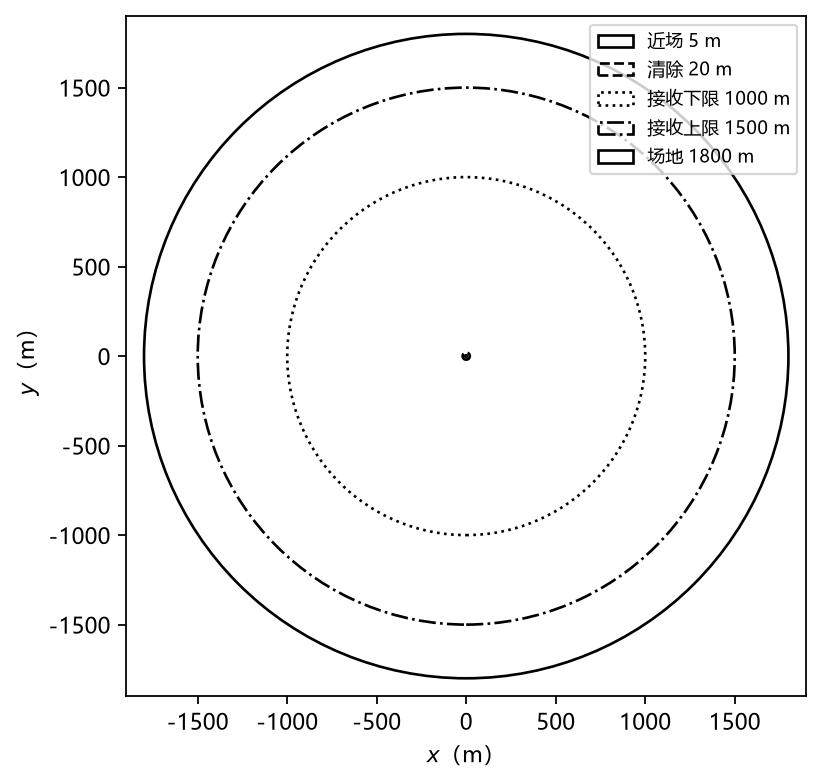
\includegraphics[width=0.72\textwidth]{figures/eda_radii.png}
\caption{场地、接收、清除与近场半径的相对尺度。}
\label{fig:radii}
\end{figure}

\begin{figure}[htbp]
\centering
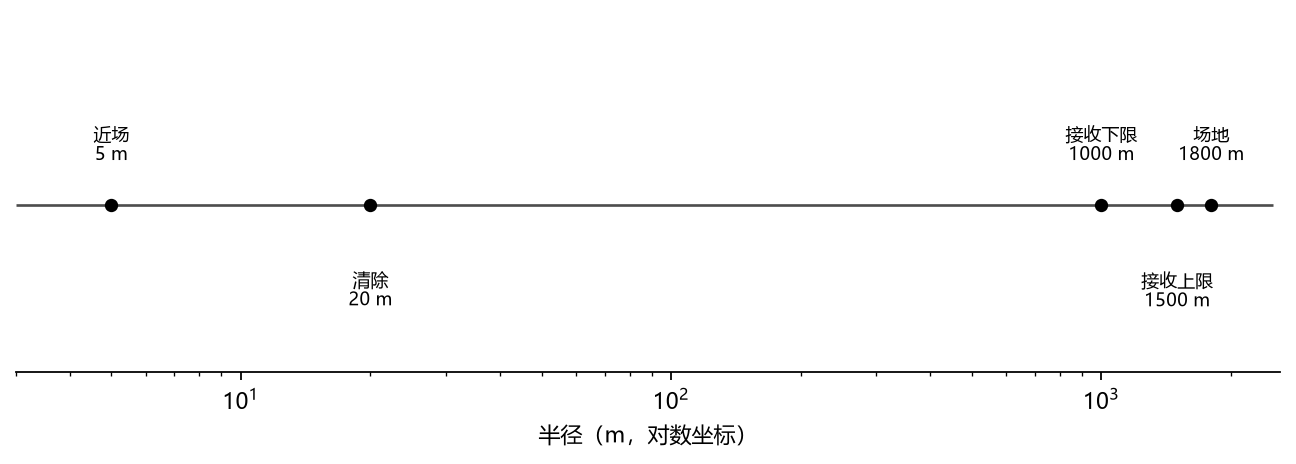
\includegraphics[width=0.92\textwidth]{figures/eda_constraint_line.png}
\caption{协议半径的对数尺度链：近场、清除、接收区间与场地半径依次增大。}
\label{fig:constline}
\end{figure}

如图\ref{fig:timecomp}所示，一次典型动作的虚拟时间中，行进200 m需要40 s，检测5 s，光学3 s，激光2 s，换台1 s。这表明移动项通常主导虚拟时钟，侦听点不宜过密，追逐时应沿用已有示向度。如图\ref{fig:protorange}所示，长度量在对数坐标下拉开：近场与清除远小于接收半径，场地半径最大。预处理不把接收区间用中点代替，而是在覆盖论证中取1000 m，在可听上界中取1500 m。

\begin{figure}[htbp]
\centering
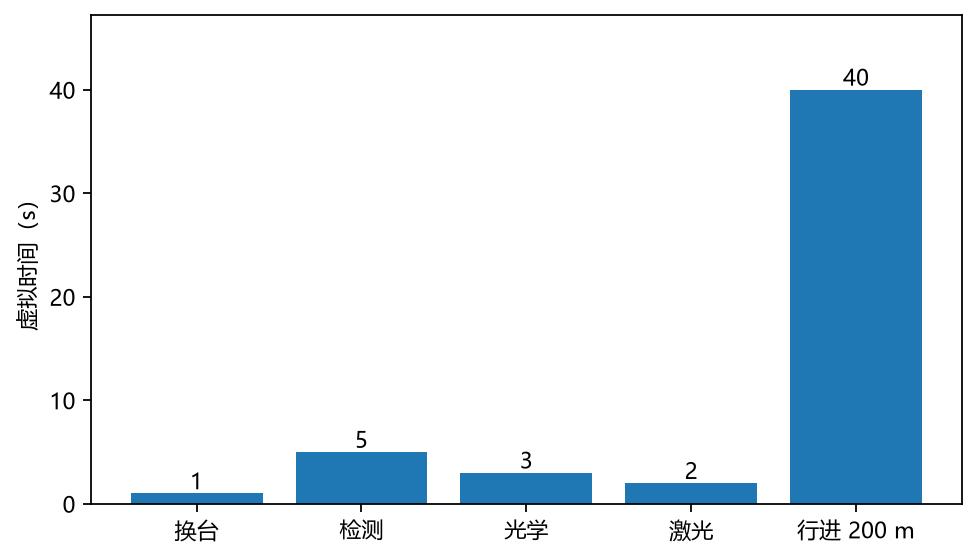
\includegraphics[width=0.82\textwidth]{figures/eda_time_components.png}
\caption{虚拟时间分量：行进200 m、检测、光学、激光与换台。}
\label{fig:timecomp}
\end{figure}

\begin{figure}[htbp]
\centering
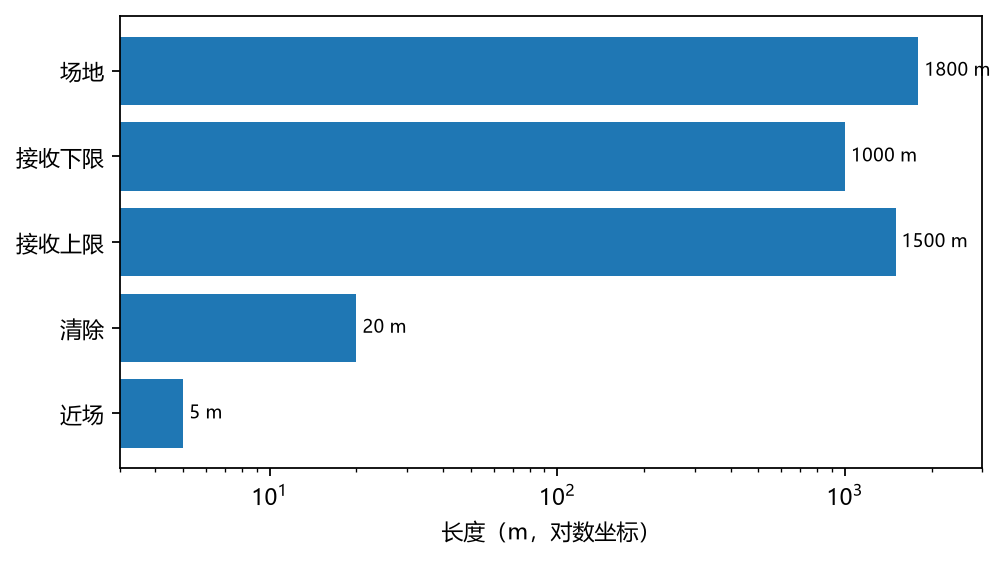
\includegraphics[width=0.72\textwidth]{figures/eda_protocol_ranges.png}
\caption{协议长度量的对数对照：仅有效接收半径为区间。}
\label{fig:protorange}
\end{figure}

\subsection{接口语义与标签口径}

模拟器通过HTTP返回\texttt{direction}、\texttt{near}、\texttt{no\_signal}以及清除结果。表\ref{tab:api}归纳四类指令的时钟含义。\texttt{direction}只提供楔形轴，不提供距离。\texttt{near}表示距离不超过5 m且在覆盖角内。\texttt{no\_signal}在全向情形可解释为超距或未进入该频道；在定向情形还可能是扇形背面。清除成功与否不能从示向度反推，只能由\texttt{/clear}的返回判定。问题三、问题四的“被清除个数比例”和“平均定位清除时间”是模拟器窗口上的统计，不是附件中的既有列。演练结束时窗口给出干扰源总数，因而比例可算；正式测试不给出总数，表1只报告清除个数与平均时间。

\begin{table}[htbp]
\centering
\caption{接口指令与虚拟时钟}
\label{tab:api}
\begin{tabular}{lll}
\toprule
指令 & 作用 & 虚拟时间增量 \\
\midrule
\texttt{/enter} & 进入场地，返回剩余现实秒数 & 0 \\
\texttt{/measure} & 在停稳点检测一个频道 & $\|P_{\mathrm{new}}-P_{\mathrm{old}}\|/5+1_{\mathrm{switch}}+5$ \\
\texttt{/clear} & 光学精定位并尝试激光清除 & $\|P_{\mathrm{new}}-P_{\mathrm{old}}\|/5+$（成功5或失败3） \\
\texttt{/exit} & 结束本次测试 & 0 \\
\bottomrule
\end{tabular}
\end{table}

每次动作使用新的请求编号，串行等待上一次返回后再发下一次；仅在重试同一中断请求时复用编号。坐标分量绝对值不得超过$2\times 10^6$ m，虚拟时间上限为100 h。实现细节见附录。

\section{问题一：交会楔形的直径与对径圆覆盖}

\subsection{机理}

测向机在检测点$S$把天线转到场强最大方向，读数$\theta$是该方向相对正东的方位。环境与仪器使读数相对真方位有不超过$1^\circ$的偏差，且同一地点的偏差固定。本文把该读数解释为凸楔形（convex wedge）的轴。其基本形式为
\begin{equation}
W(S,\theta;\varepsilon)=\bigl\{P:\delta\bigl(\tfrac{180}{\pi}\mathrm{atan2}(P_y-S_y,P_x-S_x),\,\theta\bigr)\le\varepsilon\bigr\},
\label{eq:wedge}
\end{equation}
其中圆距离$\delta(\alpha,\theta)=\min_k|\alpha-\theta-360k|$，$\varepsilon=1^\circ$为题设半误差，$P$为平面上的候选点。半角$1^\circ$远小于$90^\circ$，楔是凸的，多楔之交仍凸。这与把示向度当无误差射线、再对交点做泰勒线性化的点估计路线不同\cite{foy1976,torrieri1984}：本题要的是区域直径，不是协方差椭圆的一次实现。如图\ref{fig:halfplane}所示，轴为$\theta$，左右边界的内法向为$n_+$与$n_-$：可行点必须同时落在两条边界直线的内侧半平面。半角在图中放大以便阅读，正文始终取$1^\circ$。

\begin{figure}[htbp]
\centering
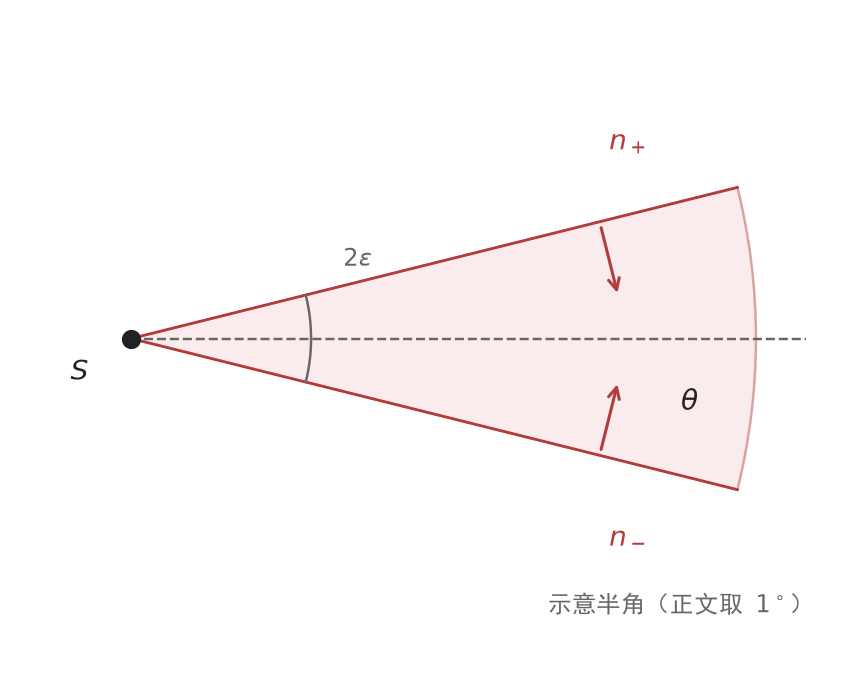
\includegraphics[width=0.78\textwidth]{figures/halfplane.png}
\caption{单站示向度楔：轴为$\theta$，左右边界的内法向为$n_+$与$n_-$。}
\label{fig:halfplane}
\end{figure}

两站中心线不平行时，四条边界射线在前方相交，得到有界四边形。如图\ref{fig:wedgeint}所示，左幅是$1^\circ$真半角的两站楔，交会区在本图尺度下缩为一点，右幅把该点放大成定位四边形。1500 m距离圆远大于该视窗，正交例的交会区未与距离圆相交。三站及以上可以把$\Omega$削成锐角三角形或六边形。锐角三角形的外接圆半径大于最长边的一半，这正是Jung等号的几何来源\cite{jung1901}。如图\ref{fig:jungschema}所示，左侧最小包围圆明显大于以一边为直径的圆，右侧对径圆恰好包住钻石。这表明对径圆覆盖不是恒真命题。

\begin{figure}[htbp]
\centering
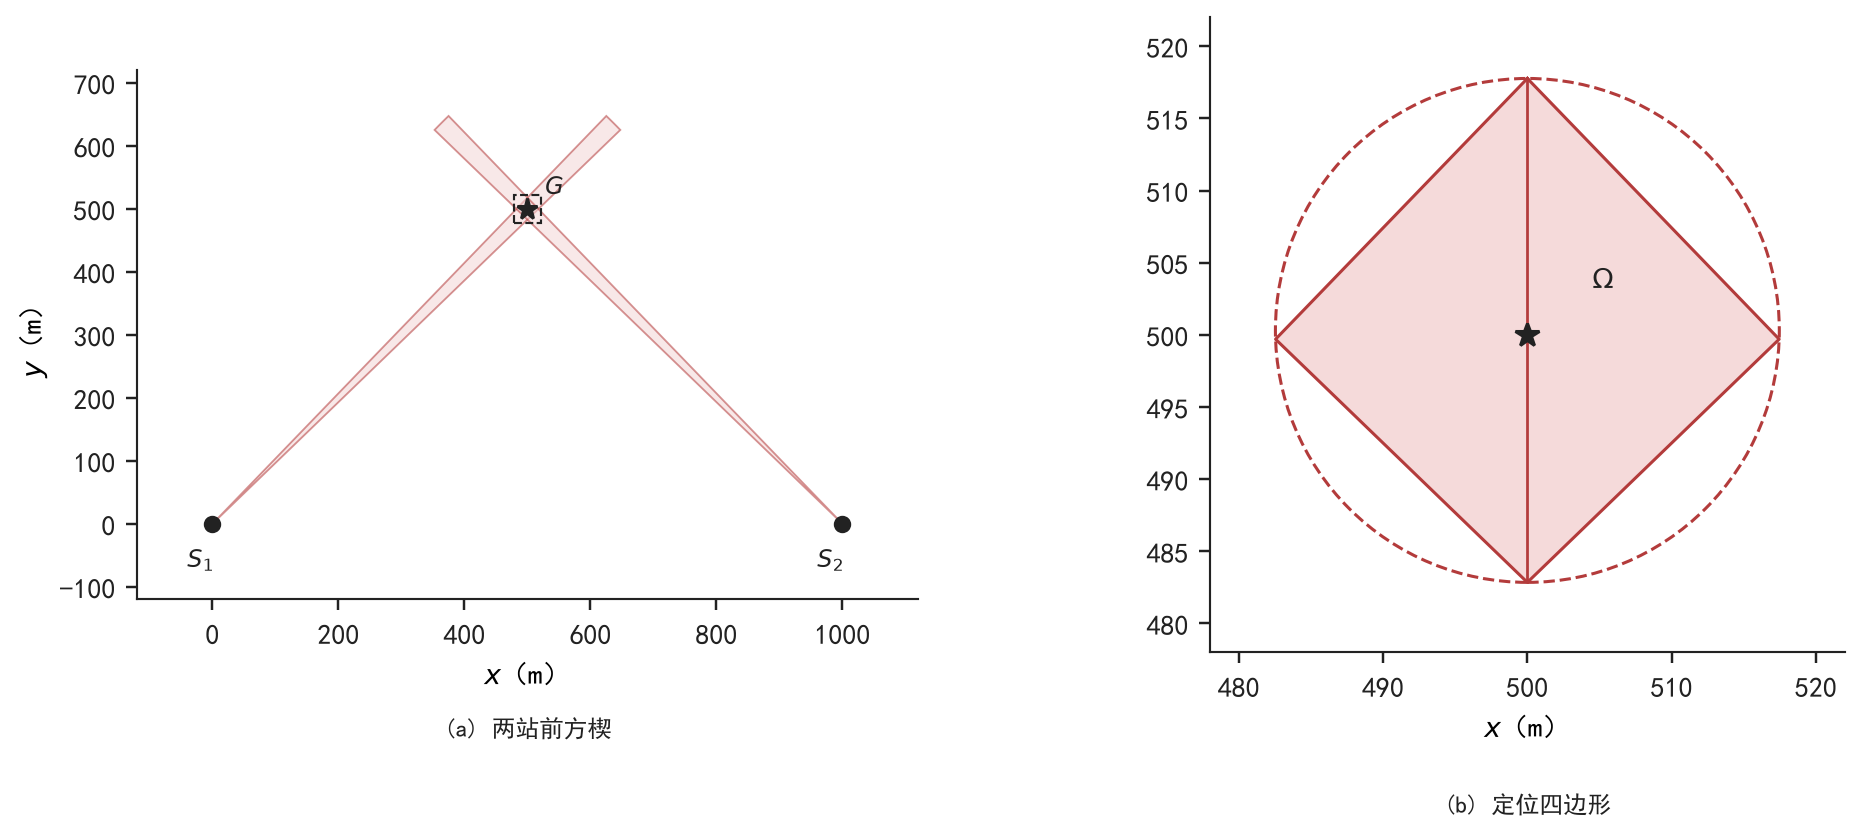
\includegraphics[width=0.82\textwidth]{figures/wedge_intersect.png}
\caption{两站前方楔形之交构成定位区域$\Omega$。左：真半角$1^\circ$；右：交会区放大。}
\label{fig:wedgeint}
\end{figure}

\begin{figure}[htbp]
\centering
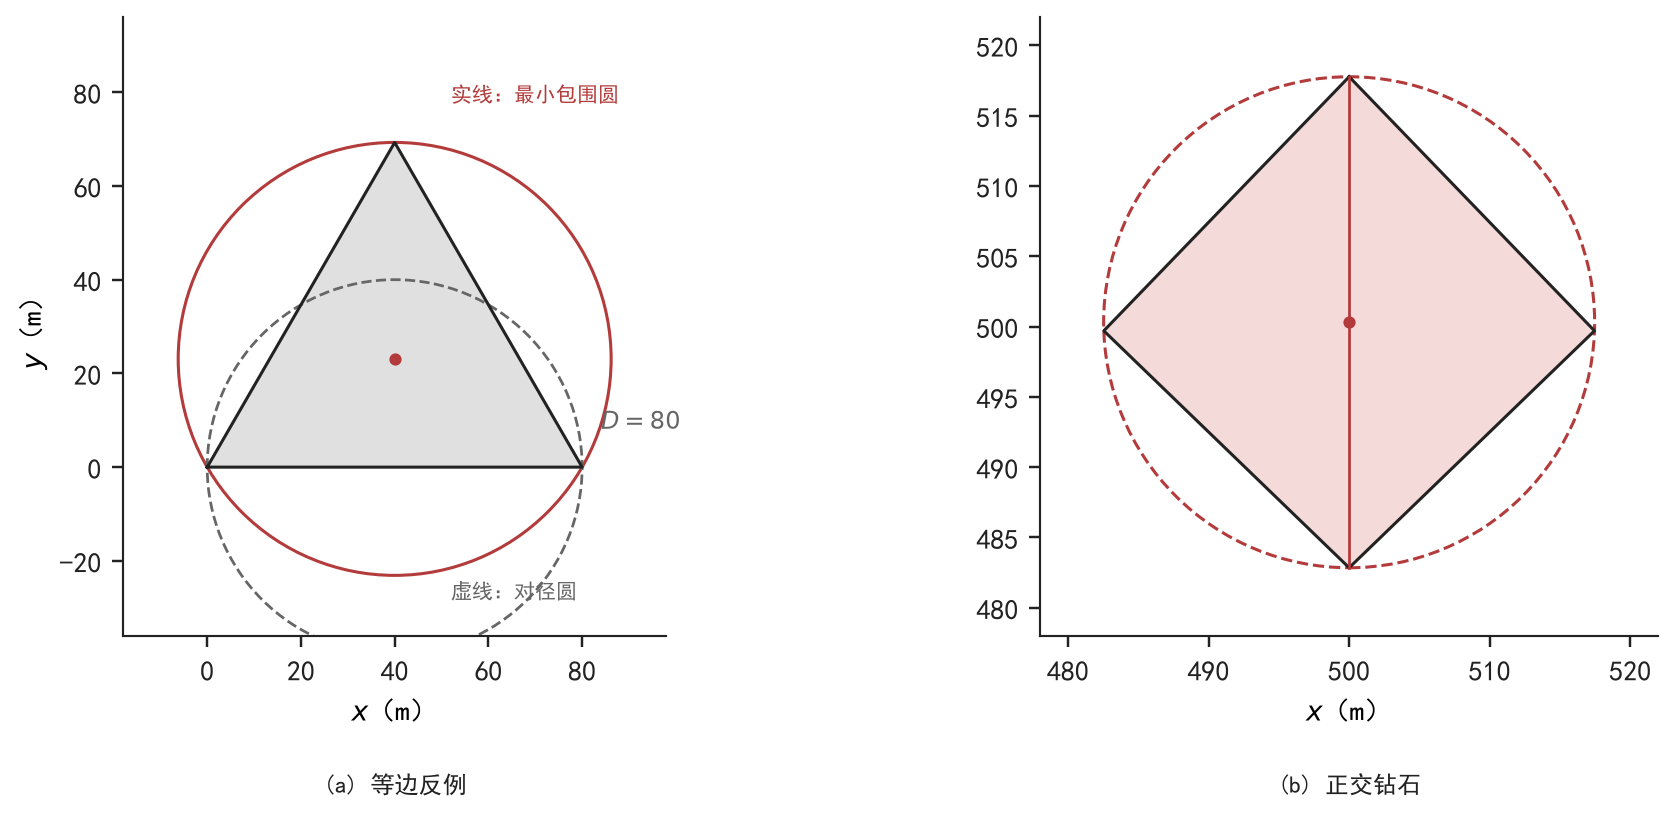
\includegraphics[width=0.82\textwidth]{figures/jung_vs_diamond.png}
\caption{对径圆覆盖不是恒真：等边三角形失败，钻石四边形成功。}
\label{fig:jungschema}
\end{figure}

\subsection{模型}

楔的半平面写法便于裁剪。记左边界方位$\phi_+=\theta+\varepsilon$，右边界方位$\phi_-=\theta-\varepsilon$，对应单位方向$u=(\cos\phi,\sin\phi)$。指向楔内的法向为
\begin{equation}
n_+=(\sin\phi_+,-\cos\phi_+),\qquad n_-=(-\sin\phi_-,\cos\phi_-).
\label{eq:normals}
\end{equation}
点$P$落在楔内当且仅当$n_\pm\cdot(P-S)\ge 0$。定位多边形由Sutherland--Hodgman半平面裁剪（polygon clipping）得到。其基本形式为：从足够大的正方形出发，依次用半平面$n\cdot x\ge c$裁去外侧顶点并插入边界交点，输出仍为凸多边形\cite{sutherland1974}。若顶点落在人工大盒边界上，则判定$\Omega$无界，有限直径圆不能覆盖。干扰源在场地内时再交圆盘$\mathbb{D}(0,1800)$；已测到信号时再交半径1500 m的距离球。圆盘与距离球用切线半平面多边形逼近后同样裁剪。

算法步骤如下。

\begin{enumerate}
\item 读入检测点与示向度$\{(S_i,\theta_i)\}$，对每一站构造两条半平面。
\item 自大正方形起做半平面裁剪，得到凸多边形顶点；必要时再交场地圆盘与距离球。
\item 若顶点落在人工大盒边界上，判定无界，直径为$+\infty$，有限对径圆不能覆盖。
\item 否则计算
\begin{equation}
D=\max_{i<j}\|v_i-v_j\|.
\label{eq:dvert}
\end{equation}
\item 对每一对径点对$\{A,B\}$（$\|A-B\|=D$），检验其余顶点是否落入以$AB$为直径的闭圆盘。由Thales定理，这等价于$\angle APB\ge 90^\circ$。
\item 等价地，用Welzl算法计算最小包围圆（smallest enclosing circle）半径$R_{\mathrm{sec}}$\cite{welzl1991}。其基本形式为在顶点集上维护当前圆，遇圆外点则把该点固定到边界并递归，覆盖当且仅当
\begin{equation}
2R_{\mathrm{sec}}\le D.
\label{eq:cover}
\end{equation}
\end{enumerate}

Jung上界$R_{\mathrm{sec}}\le D/\sqrt{3}$只说明覆盖可能失败，并不给出失败的充分条件；失败必须由\eqref{eq:cover}的直接检验确认。无约束直线求交若不检查射线参数，会在对向示向度下给出后方交点。后方交点不满足式\eqref{eq:wedge}，不属于定位区域。本文以半平面裁剪为准。

\subsection{估计与检验}

题面未给检测点坐标。检验用文中写明的合成站点，种子为2026。正交交会例取$S_1=(0,0)$示向度$45^\circ$，$S_2=(1000,0)$示向度$135^\circ$，真源在$(500,500)$。等边反例取边长80 m的三角形；三站楔在等边核周围交出六边形。两站Monte Carlo在场地内抽样源与站点，叠加$\pm 1^\circ$读数后计算有界样本的覆盖率：请求400个样本，全部有界，其中382个对径圆覆盖，覆盖率$382/400=0.955$。直方图、散点与附录CSV使用这同一组400行，不是另行抽取的子样本。辅助直线交点与半平面顶点的最大距离用于核对正交例。

\subsection{结果}

由表\ref{tab:q1head}可知，正交交会例得到4个顶点，直径34.92 m，最小包围圆半径17.46 m，恰为直径的一半，对径圆覆盖取1，面积为609.36 m$^2$。辅助直线交点与半平面顶点的最大误差为0，说明在正交交叉这种“前方可见”的构型上，两种求交一致。如图\ref{fig:q1ex}所示，左幅给出两站与真源的相对位置，交会区在千米尺度下缩为一点，故用红框标出右幅视窗；右幅把定位四边形和对径圆放大到四十米视窗：四边形几乎是对径圆的内接钻石。这表明覆盖判定与目视一致。表\ref{tab:q1vert}列出四个顶点坐标，直径在相对的顶点对上取得。

\begin{table}[htbp]
\centering
\caption{问题一合成正交交会例的几何量}
\label{tab:q1head}
\begin{tabular}{lr}
\toprule
量 & 取值 \\
\midrule
顶点个数 & 4 \\
直径 / m & 34.92 \\
最小包围圆半径 / m & 17.46 \\
对径圆覆盖 & 1 \\
面积 / m$^2$ & 609.36 \\
辅助顶点最大误差 / m & 0 \\
比值 $R_{\mathrm{sec}}/D$ & 0.500 \\
\bottomrule
\end{tabular}
\end{table}

\begin{table}[htbp]
\centering
\caption{正交交会例的定位多边形顶点}
\label{tab:q1vert}
\begin{tabular}{crr}
\toprule
编号 & $x$ / m & $y$ / m \\
\midrule
1 & 500.000 & 517.765 \\
2 & 482.550 & 499.695 \\
3 & 500.000 & 482.844 \\
4 & 517.450 & 499.695 \\
\bottomrule
\end{tabular}
\end{table}

\begin{figure}[htbp]
\centering
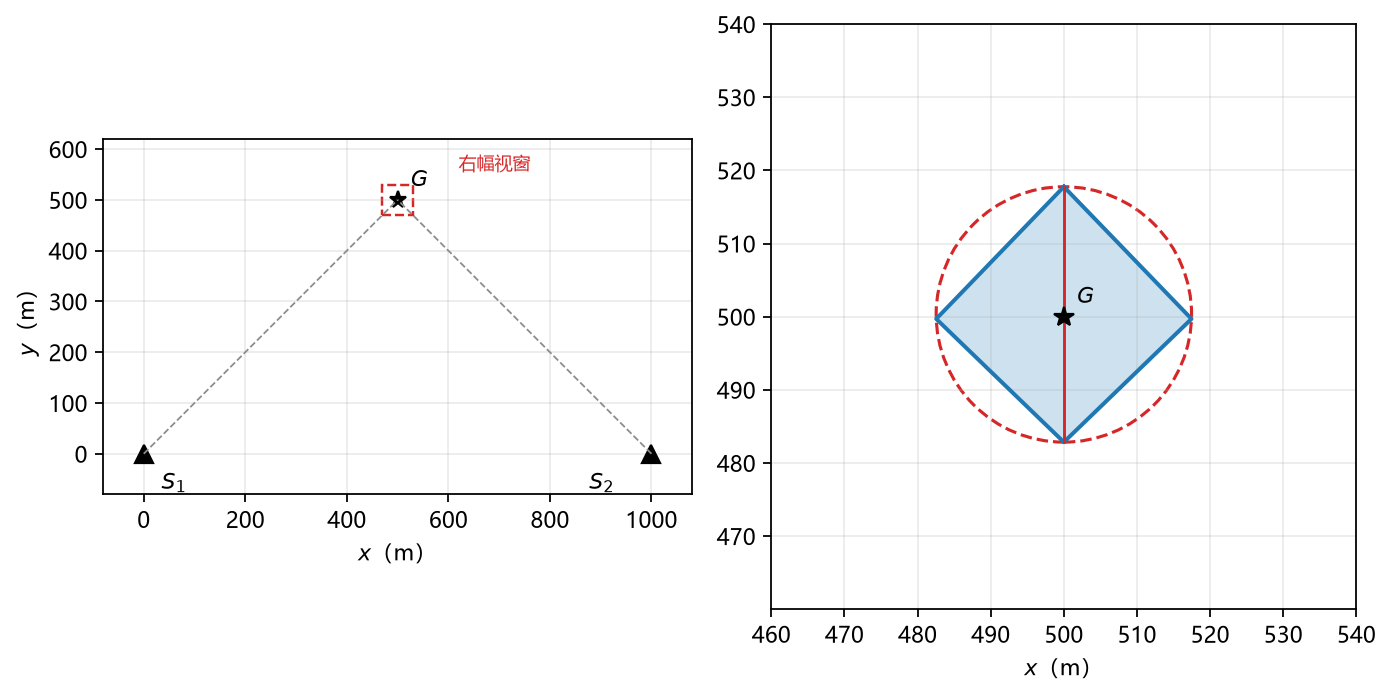
\includegraphics[width=0.98\textwidth]{figures/q1_example_polygon.png}
\caption{正交交会合成例。左：两站与真源；右：定位四边形及其对径圆。}
\label{fig:q1ex}
\end{figure}

由表\ref{tab:q1cover}可知，未裁剪的两站有界样本384个全部被对径圆覆盖，覆盖率为1；与场地及距离球相交后，长条钻石被切断成略锐的三角形，400个有界样本中382个覆盖，覆盖率为0.955。边长80 m的等边三角形最小包围圆半径46.19 m，大于40 m，覆盖取0。三站楔的六边形同样覆盖取0，直径93.32 m，最小包围圆半径47.13 m。如图\ref{fig:jungschema}所示，左侧虚线对径圆不能包住等边三角形，右侧对径圆包住钻石。这表明“以直径为直径的圆能否覆盖”必须作为布尔输出，而不能预先回答“能”。

\begin{table}[htbp]
\centering
\caption{对径圆覆盖的正例与反例}
\label{tab:q1cover}
\begin{tabular}{lrr}
\toprule
情形 & 覆盖 & 说明 \\
\midrule
两站未裁剪有界样本 & 1 & 384个有界样本 \\
两站裁剪后 & 0.955 & 400个有界样本，其中382个覆盖 \\
等边三角形 & 0 & 边长80 m \\
三站六边形 & 0 & 反例 \\
\bottomrule
\end{tabular}
\end{table}

如图\ref{fig:q1mc}所示，裁剪后两站直径的直方图来自上述400个有界样本：中位直径137.95 m，显著大于清除直径40 m；右幅覆盖382个、未覆盖18个，与覆盖率0.955一致。这表明两站交会通常还不能一次清除，需要问题二把第二站放到近乎正交的位置，或者在追逐中继续加密测点。如图\ref{fig:jungratio}所示，左幅给出残差$R_{\mathrm{sec}}-D/2$：覆盖样本落在零线，18个未覆盖样本的残差为正，最大比值$R_{\mathrm{sec}}/D=0.5005$；右幅给出面积随直径的散点，长条区域面积并不随直径线性增长。

\begin{figure}[htbp]
\centering
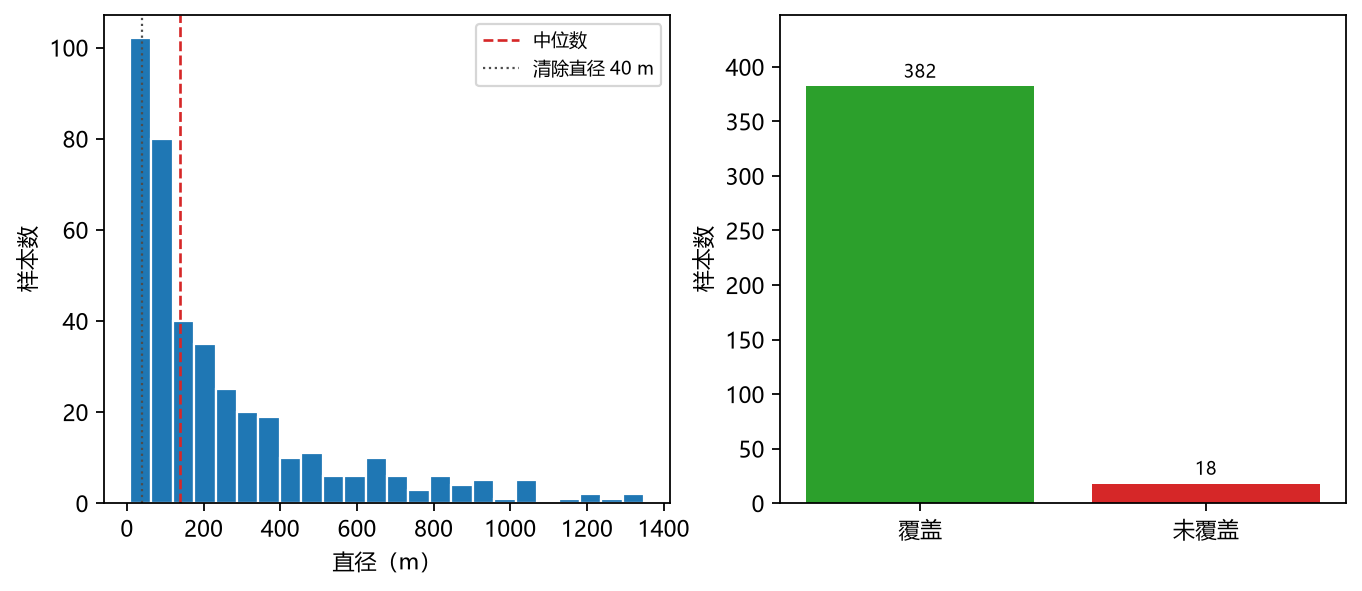
\includegraphics[width=0.92\textwidth]{figures/q1_mc_diameter.png}
\caption{两站裁剪后400个有界样本的直径分布与覆盖计数（382覆盖、18未覆盖）。}
\label{fig:q1mc}
\end{figure}

\begin{figure}[htbp]
\centering
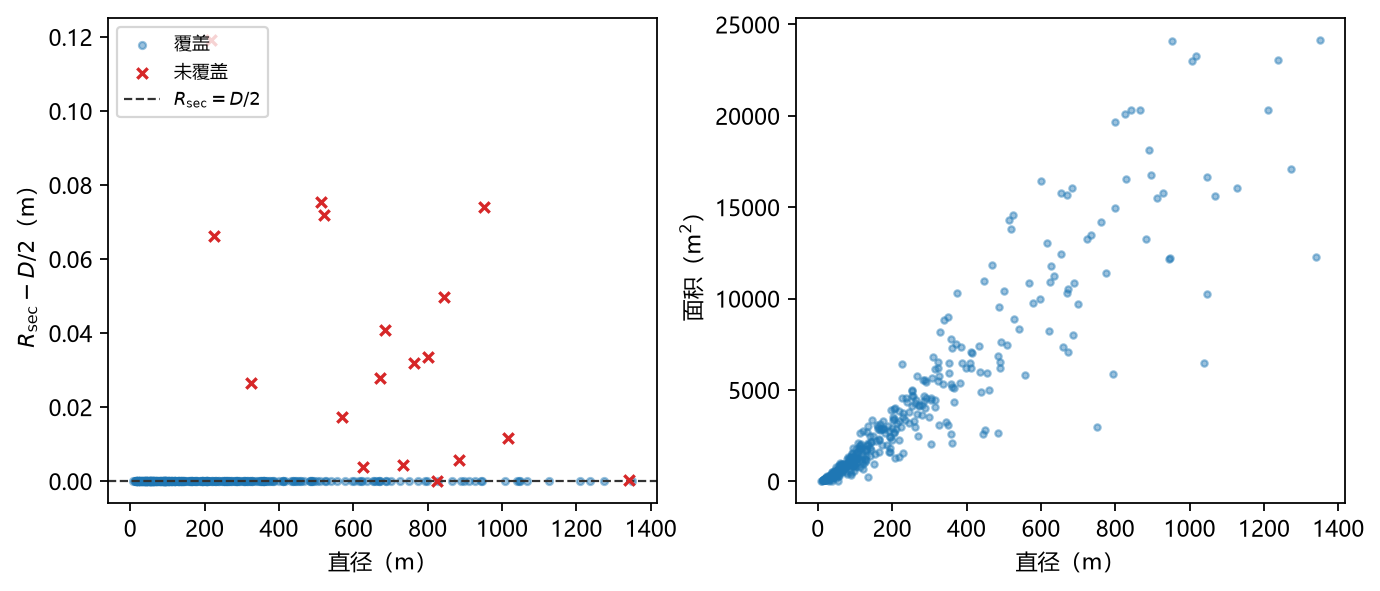
\includegraphics[width=0.92\textwidth]{figures/q1_jung_ratio_area.png}
\caption{左：400个有界样本的残差$R_{\mathrm{sec}}-D/2$；右：定位多边形面积与直径。}
\label{fig:jungratio}
\end{figure}

\subsection{诊断}

第一，直径算法在无界楔交上必须返回无穷，否则会把大盒边长误当作场地尺度。第二，辅助直线交点在正交例上与裁剪顶点误差为0，不能推广到对向示向度；对向时后方交点必须丢弃。第三，覆盖判定对顶点扰动稳定，因为正交例的$R_{\mathrm{sec}}/D$几乎恰好为$1/2$。第四，题目问“能否覆盖”的语言容易被读成恒真，等边反例说明必须保留布尔输出。第五，合成坐标不是赛题真值，算法对一般站点组可执行，数值只对写明的例子成立。第六，场地裁剪会把覆盖率从1降到0.955，正文报告覆盖结论时必须声明是否与场地相交。

\section{问题二：第二检测点的正交基线与候选带}

\subsection{机理}

第一站把源限制在窄楔$\Omega_1$内。楔的宽度在距离$r_G$处约为$2r_G\sin\varepsilon\approx 2r_G\varepsilon$，沿轴却可延伸到接收半径上界。第二站的任务是把这条长带切成直径可与清除圆相比的有界多边形。若$S_2$落在轴上，交角趋于$0^\circ$或$180^\circ$，切出来的仍是长条。Nardone等对纯方位可观测性的分析表明，观测器必须离开视线\cite{nardone1984}；Dogancay指出线性最小二乘在纯方位上有几何偏差\cite{dogancay2005}。因此把第二站写成正交基线（orthogonal baseline）。其基本形式为$S_2=S_1+r u_{\theta}+t v_{\theta}$，其中$u_{\theta}$为示向度单位向量，$v_{\theta}$为左转法向，$t$可正可负。横向偏移$t$是决策变量，而不是可有可无的扰动。

对轴上假设点$G=S_1+r_G u_{\theta}$，第二站$S_2=S_1+r u_{\theta}+t v_{\theta}$的交角满足
\begin{equation}
\cos\psi=\frac{r_G-r}{\sqrt{(r_G-r)^2+t^2}}.
\label{eq:psi}
\end{equation}
$\psi=90^\circ$当且仅当$r=r_G$。$\psi\in[45^\circ,135^\circ]$当且仅当$|r-r_G|\le|t|$。小角近似\eqref{eq:smallang}给出与40 m清除直径同量级的横向尺度，避免把$t$取得过小。

\subsection{模型}

如图\ref{fig:s2schema}所示，第二站写成$S_2=S_1+r u_{\theta}+t v_{\theta}$，候选比较在轴两侧进行，而不是绕$S_1$的圆环。对轴上$r_G\in[r_{\mathrm{lo}},r_{\mathrm{hi}}]$，交角覆盖写成两条引理。

\textbf{引理（轴上$[45^\circ,135^\circ]$覆盖）。} 假设$G$落在示向度轴上且$r_G\in[r_{\mathrm{lo}},r_{\mathrm{hi}}]$。则对该区间内一切$r_G$都有$\psi\in[45^\circ,135^\circ]$，当且仅当
\begin{equation}
|t|\ge\max\bigl(|r-r_{\mathrm{lo}}|,\,|r_{\mathrm{hi}}-r|\bigr).
\label{eq:psiband}
\end{equation}
取$r_{\mathrm{lo}}=5$ m、$r_{\mathrm{hi}}=1500$ m、$r=800$ m，得$|t|\ge 795$ m。

\textbf{引理（轴上$\psi\ge 45^\circ$覆盖）。} 同一假设下，$r_G\le r$时$\psi\ge 90^\circ\ge 45^\circ$自动成立。故对该区间内一切$r_G$都有$\psi\ge 45^\circ$，当且仅当
\begin{equation}
|t|\ge\max(0,\,r_{\mathrm{hi}}-r).
\label{eq:psi45}
\end{equation}
在$r=800$ m得$|t|\ge 700$ m。取$|t|=700$ m时，$\psi(1500)=45^\circ$，$\psi(5)\approx 138.64^\circ>135^\circ$。近端瘦钝角是本引理的残差，不是$[45^\circ,135^\circ]$覆盖。离轴$\pm 1^\circ$不在这两条引理范围内。

交付点取轴上$\psi\ge 45^\circ$覆盖点$(r,|t|)=(800,700)$ m。网格取$r\in[400,1400]$、$|t|\in[150,1000]$，对$\Omega_1$的径向--角度样本计算事后直径、交角和可听比例；该网格只作比较。网格分位点$(800,690.9)$ m使远轴$\psi(1500)\approx 44.63^\circ<45^\circ$，因而不是覆盖点。过样本形心的垂线把中位直径压得更小，但其直径90\%分位超过90 m，且不覆盖全轴，同样不是方案。两侧中选择离当前机器狗更近、更不远离场地的一点。若第二站\texttt{no\_signal}，改测另一侧$-t$，再沿示向度前进，而不是沿轴退回。问题二的交付点用于轴上交角覆盖；问题三全向局部化不把该点当作默认第二站。

\begin{figure}[htbp]
\centering
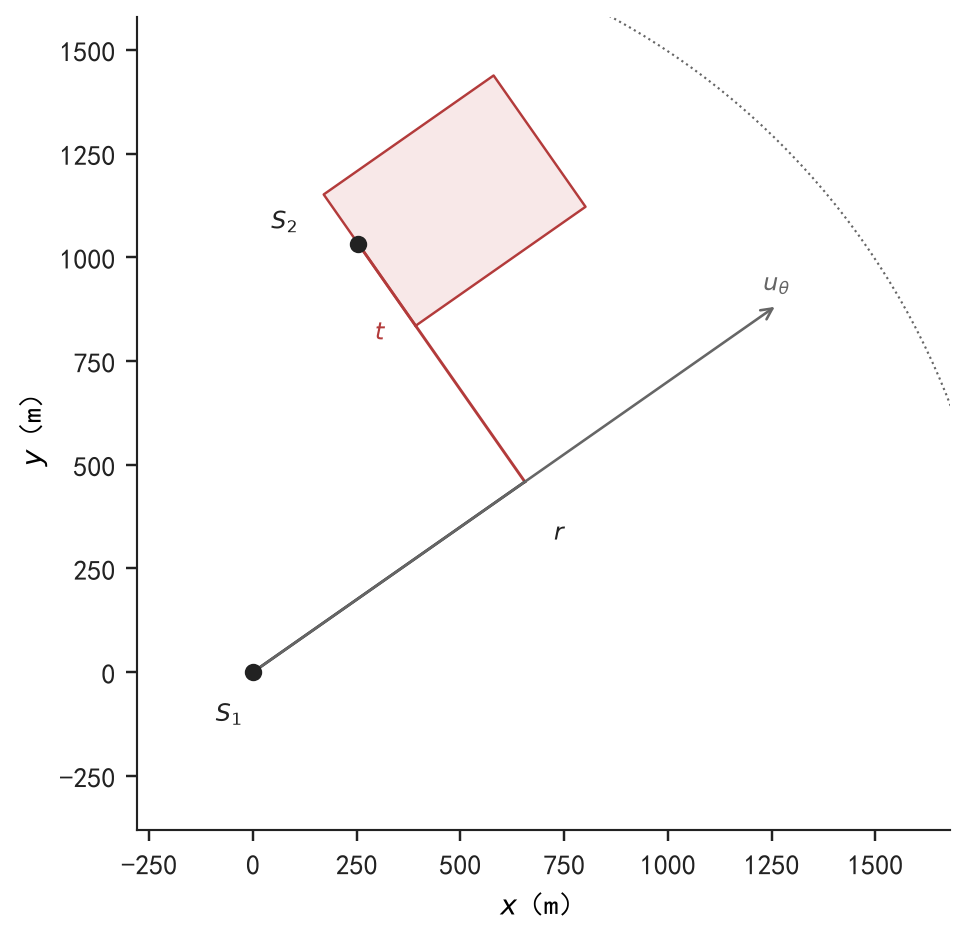
\includegraphics[width=0.72\textwidth]{figures/second_station.png}
\caption{第二站离开第一示向度轴：轴向距离$r$、横向偏移$t$。交付点$|t|=700$ m由轴上$\psi\ge 45^\circ$覆盖给出；网格分位点$|t|=690.9$ m只作比较。}
\label{fig:s2schema}
\end{figure}

\subsection{估计与检验}

交付点、网格分位点与带宽覆盖点在同一套楔形交算法上计算，种子仍为2026。第一站取$S_1=(0,0)$、示向度$35^\circ$，在楔内作径向--角度样本，样本容量$n=70$。灵敏度固定轴向距离$r=1100$ m。横向偏移依次取$200$、$350$、$500$、$650$、$800$、$1000$ m。楔半角扫描固定在同一轴向的$t=500$ m，另取$0.5^\circ$、$1^\circ$与$1.5^\circ$，对应剖面$(r,t)=(1100,500)$ m，而不是交付点$(800,700)$ m，也不是网格分位点$(800,690.9)$ m。一次清除定义为对径圆覆盖且$D\le 40$ m，或最小包围圆半径本身不超过20 m。

\subsection{结果}

由表\ref{tab:q2des}可知，网格分位点取$r=800$ m、$|t|=690.9$ m，事后直径中位数48.27 m，90\%分位88.94 m，交角中位数$93.85^\circ$。同一套楔内径向--角度样本$n=70$，其中1000 m可听$65/70$（0.93），一次清除$15/70$（$\eta_1=0.21$）。该分位点不是交付点：远轴$\psi(1500)\approx 44.63^\circ<45^\circ$。由表\ref{tab:q2cmp}可知，交付点$(800,700)$ m在同一$n=70$样本上中位直径48.29 m、可听$65/70$，并覆盖轴上$\psi\ge 45^\circ$；$[45^\circ,135^\circ]$覆盖点$(800,795)$ m把可听降到$55/70$，中位直径48.82 m。过样本形心的垂线中位直径46.43 m更小，但直径90\%分位93.69 m超过90 m，且不覆盖全轴。网格比较带为
\[
r\in[800,1300]\,\mathrm{m},\qquad |t|\in[459.1,845.5]\,\mathrm{m},
\]
面积约$3.71\times 10^{5}$ m$^2$，其中$(800,459)$已使远轴$\psi<45^\circ$，故该带不是覆盖集。表\ref{tab:q2xy}给出分位点与交付点在$\theta=35^\circ$时的两侧坐标：从$S_1$走到交付点约1063 m。如图\ref{fig:heatD}所示，事后直径中位数在小$t$和大$r$同时出现时迅速变坏，红框为比较带，星号为网格分位点。如图\ref{fig:heatpsi}所示，比较带大致落在$90^\circ$附近的暖色区域。这表明取较大横向偏移是为了把交角留在可观测区间，而不是把第二站贴在第一示向度轴上。

\begin{table}[htbp]
\centering
\caption{问题二网格分位点与比较带（$n=70$，不是覆盖集）}
\label{tab:q2des}
\begin{tabular}{lr}
\toprule
量 & 取值 \\
\midrule
轴向距离 / m & 800 \\
网格横向偏移 / m & 690.9 \\
交付横向偏移 / m & 700 \\
分位点直径中位数 / m & 48.27 \\
分位点直径90\%分位 / m & 88.94 \\
分位点交角中位数 / 度 & 93.85 \\
楔内径向--角度样本 $n$ & 70 \\
分位点1000 m可听 & $65/70$（0.93） \\
分位点一次清除 $\eta_1$ & $15/70$（0.21） \\
比较带$r$下限 / m & 800 \\
比较带$r$上限 / m & 1300 \\
比较带$|t|$下限 / m & 459.1 \\
比较带$|t|$上限 / m & 845.5 \\
\bottomrule
\end{tabular}
\end{table}

\begin{table}[htbp]
\centering
\caption{分位点与交付点在示向度$35^\circ$时的两侧坐标}
\label{tab:q2xy}
\begin{tabular}{lrrr}
\toprule
点 & $x$ / m & $y$ / m & 至$S_1$距离 / m \\
\midrule
网格 $+t=690.9$ & 259.03 & 1024.82 & 1057.05 \\
网格 $-t$ & 1051.61 & $-107.10$ & 1057.05 \\
交付 $+t=700$ & 253.82 & 1032.28 & 1063.01 \\
交付 $-t=700$ & 1056.82 & $-114.56$ & 1063.01 \\
\bottomrule
\end{tabular}
\end{table}

\begin{table}[htbp]
\centering
\caption{同一$n=70$样本上第二站候选的比较（启发式不是方案）}
\label{tab:q2cmp}
\begin{tabular}{lrrrrr}
\toprule
点 & $|t|$ / m & $\psi\ge 45^\circ$ & $[45^\circ,135^\circ]$ & 中位直径 / m & 1000 m可听 \\
\midrule
网格分位 & 690.9 & 0 & 0 & 48.27 & $65/70$ \\
交付（$\psi\ge 45^\circ$） & 700 & 1 & 0 & 48.29 & $65/70$ \\
带宽覆盖 & 795 & 1 & 1 & 48.82 & $55/70$ \\
形心垂线 & --- & 0 & 0 & 46.43 & --- \\
\bottomrule
\end{tabular}
\end{table}

\begin{figure}[htbp]
\centering
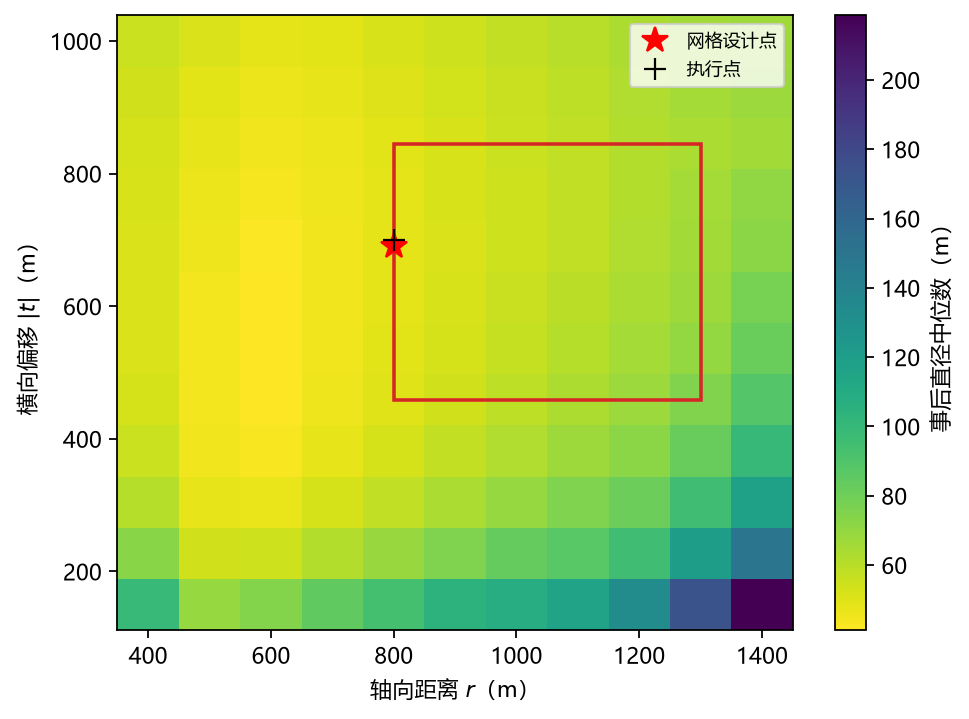
\includegraphics[width=0.82\textwidth]{figures/q2_median_D_heatmap.png}
\caption{事后直径中位数随$(r,|t|)$的变化。红框为比较带，星号为网格分位点；交付点在$|t|=700$ m。}
\label{fig:heatD}
\end{figure}

\begin{figure}[htbp]
\centering
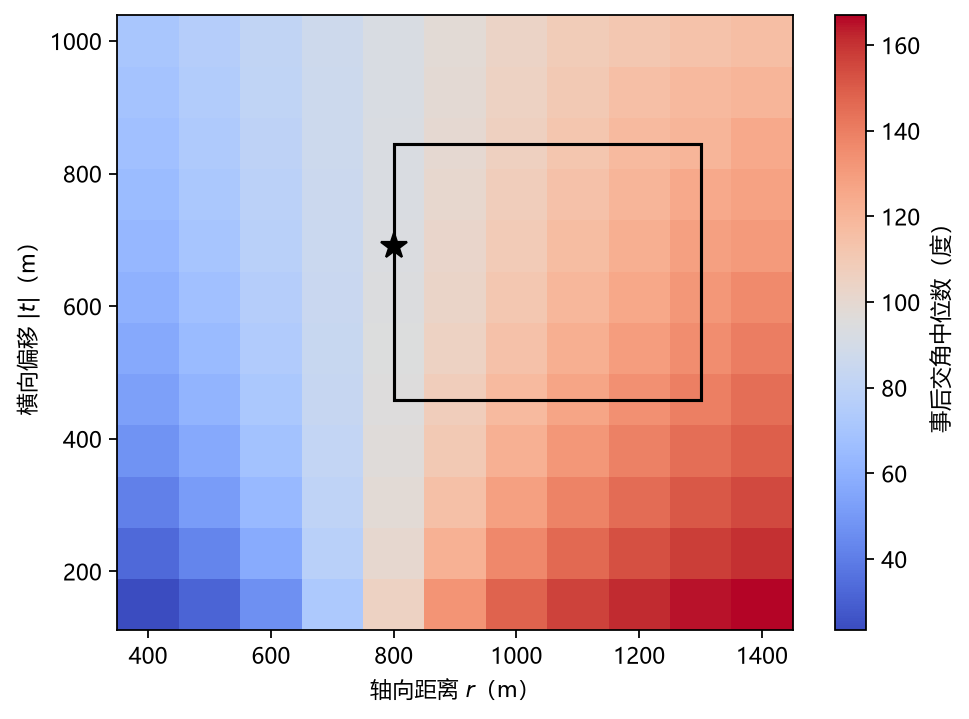
\includegraphics[width=0.82\textwidth]{figures/q2_psi_heatmap.png}
\caption{事后交角中位数随$(r,|t|)$的变化。}
\label{fig:heatpsi}
\end{figure}

由表\ref{tab:q2sens}可知，固定$r=1100$ m时，$t=200$ m的直径中位数为93.12 m，$t=800$ m为58.03 m，相差35.09 m。决策因此取较大横向偏移而不是贴轴。$t=1000$ m时1000 m可听比例降到0.07，直径中位数回升到60.29 m，说明横向不能无限加大。如图\ref{fig:sens}所示，左幅中位直径随$t$先降后升，右幅可听比例在$t>800$ m后迅速下降；40 m参考线表明，题设$1^\circ$下单次两站交会通常还不能保证一次清除。如图\ref{fig:errsweep}所示，楔半角扫描固定在$(r,t)=(1100,500)$ m：半角从$0.5^\circ$增到$1.5^\circ$，中位直径从30.99 m增到92.65 m，一次清除从1变为0。该0--1翻转属于灵敏度剖面$(1100,500)$ m；网格分位点$(r,t)=(800,690.9)$ m的一次清除比例为$\eta_1=0.21$，交付点是另一组坐标$(800,700)$ m。这表明在$(1100,500)$ m处，题设$1^\circ$恰好卡在一次清除的边界上。

\begin{table}[htbp]
\centering
\caption{固定$r=1100$ m时横向偏移的灵敏度}
\label{tab:q2sens}
\begin{tabular}{rrrrr}
\toprule
$t$ / m & 中位直径 / m & 90\%分位 / m & 交角中位 / 度 & 1000 m可听 \\
\midrule
200 & 93.12 & 166.34 & 149.85 & 0.93 \\
350 & 70.15 & 114.93 & 134.54 & 0.93 \\
500 & 61.87 & 89.43 & 124.62 & 0.86 \\
650 & 58.96 & 78.12 & 118.01 & 0.79 \\
800 & 58.03 & 74.80 & 113.40 & 0.64 \\
1000 & 60.29 & 74.92 & 109.11 & 0.07 \\
\bottomrule
\end{tabular}
\end{table}

\begin{figure}[htbp]
\centering
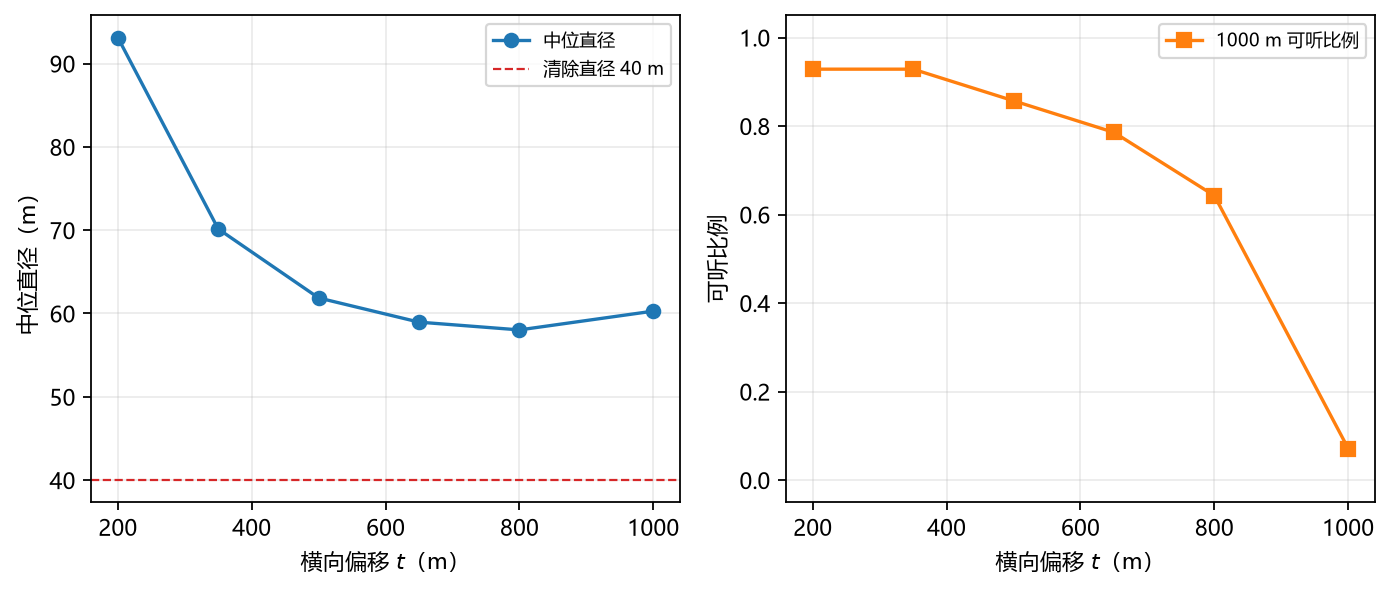
\includegraphics[width=0.98\textwidth]{figures/q2_sensitivity.png}
\caption{左：横向偏移对中位直径的影响；右：1000 m可听比例随横向偏移下降。}
\label{fig:sens}
\end{figure}

\begin{figure}[htbp]
\centering
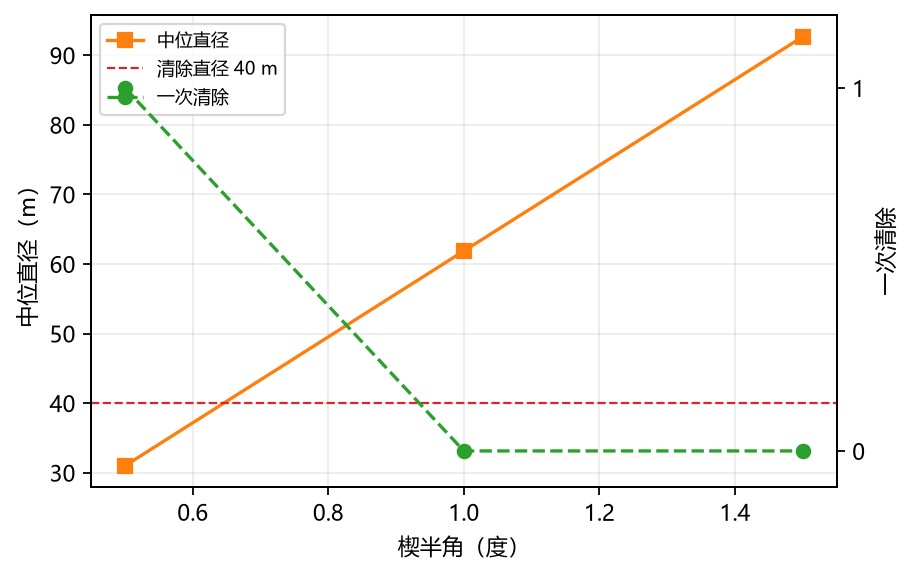
\includegraphics[width=0.72\textwidth]{figures/q2_err_sweep.png}
\caption{楔半角对中位直径与一次清除的影响，剖面$(r,t)=(1100,500)$ m。橙实线为中位直径，绿虚线为一次清除，红虚线为清除直径40 m。}
\label{fig:errsweep}
\end{figure}

\subsection{诊断}

有效接收半径未知，不能保证对$\Omega_1$内每一点都听到；交付点用1500 m上界给出$\psi\ge 45^\circ$覆盖，并用1000 m可听比例报告可听代价。第一站很靠场地边缘时，$r=800$ m可能把$S_2$送出盘外，协议允许盘外检测，移动耗时仍按直线距离计算。网格分位点的一次清除比例$\eta_1=0.21$，因而两站交会通常还不能一次清除。问题三的修订策略先完成发现，再用距离上界收缩给出有限步清除证书。$t=200$ m把交角中位数推到约$150^\circ$，几何接近共线，直径中位数超过90 m，该点不能作为覆盖点。$|t|=700$ m由式\eqref{eq:psi45}给出，不是把$690.9$ m圆整；近端$\psi(5)\approx 138.64^\circ$是该引理的残差。问题三全向追逐不把该交付点当作默认第二站。

\section{问题三：有限侦听覆盖与有界收缩清除}

\subsection{模型与策略}

场地为闭圆盘$\mathbb A=\overline{\mathbb D}(0,1800)$。每个源的位置和频道固定，频道互异，源数$10\le N\le16$。对源$G$，有效接收半径$R_G\in[1000,1500]$；全向测量可听当且仅当检测点与源的距离不超过$R_G$。测向误差满足$|\alpha|\le1^\circ$，不要求独立、均匀或无偏，同一点重复测量也不被当作新信息。光学清除只要求距离不超过20 m；\texttt{near}表示距离不超过5 m，可以就地清除。

策略分为有限发现与有界清除两阶段。先处理原点及8个环点，每站完整扫描尚未发现的频道；仅在有严格覆盖证书时跳过该站。发现阶段不插入远距离追逐，以免覆盖任务被服务启发式反复推迟。然后对每个已发现且未清除的频道，使用示向度与距离上界逐步收缩，最后在保证进入20 m清除窗的位置清除。覆盖点的访问顺序用开放旅行商问题缩短路程，服务顺序按到下一收缩点的距离选择；这些顺序规则不改变完备性，也不声称求得全任务的全局最短时间。

虚拟时间按实际动作累加：
\begin{align}
\Delta T_{\rm measure}&=\|P_{\rm new}-P_{\rm old}\|/5
+\mathbf 1_{c\ne c_{\rm radio}}+5,\label{eq:tmeas}\\
\Delta T_{\rm clear}&=\|P_{\rm new}-P_{\rm old}\|/5+
\begin{cases}5,&\text{成功},\\3,&\text{未发现光学目标}.\end{cases}\label{eq:tclr}
\end{align}
修订算法的清除点均有距离证书，因此模型内应走成功分支；若接口返回失败，程序报告证书或模型异常，不把失败算成完成。现实程序时间与虚拟时间分别记录。

\subsection{9点侦听覆盖及其完整证明}

侦听点为
\begin{equation}
\mathcal N=\{O\}\cup\{R_k:k=0,\ldots,7\},\quad O=(0,0),\quad
R_k=1000(\cos(k\pi/4),\sin(k\pi/4)).\label{eq:q3net}
\end{equation}
定义最近站距离$d_{\mathcal N}(G)=\min_{S\in\mathcal N}\|G-S\|$。

\textbf{引理1（全向覆盖）。}在场地闭圆盘上，
\begin{equation}
\max_{G\in\mathbb A}d_{\mathcal N}(G)
=\rho=\sqrt{1800^2+1000^2-2\cdot1800\cdot1000\cos(\pi/8)}
\approx956.0511<1000.\label{eq:q3rho}
\end{equation}

\textbf{证明。}记$r=\|G\|$，$\delta\in[0,\pi/8]$为$G$与最近环点的夹角。令$\gamma=\cos(\pi/8)$、$\tau=1000/(2\gamma)\approx541.196$。若$r\le\tau$，选择原点即可使距离不超过$\tau<\rho$。若$\tau\le r\le1800$，选择最近环点$R$，由余弦定理，
\[
\|G-R\|^2=r^2+10^6-2000r\cos\delta
\le f(r):=r^2+10^6-2000\gamma r.
\]
$f$为凸函数，因此$f(r)\le\max\{f(\tau),f(1800)\}=\max\{\tau^2,\rho^2\}=\rho^2$。边界角平分点$P=1800(\cos(\pi/8),\sin(\pi/8))$到两相邻环点的距离均为$\rho$，到原点为1800，故上界可取到。证毕。

上述$r\le\tau$是证明中\emph{选择原点足以给出上界}的区间，不是所有方向上的最近站分界。固定$\delta$时，原点与最近环点等距的半径是$1000/(2\cos\delta)$；例如$G=(520,0)$的最近环点距其480 m，比原点近。另须区分覆盖半径：8个环点在原点的最近距离为1000 m，所以它们不能以$\rho$为半径覆盖原点，但可以用闭1000 m盘覆盖原点；事实上8环以闭1000 m盘已覆盖场地。保留原点扫描利用了题设初始位置，且使最大最近距离降至$\rho$。

\begin{figure}[htbp]
\centering
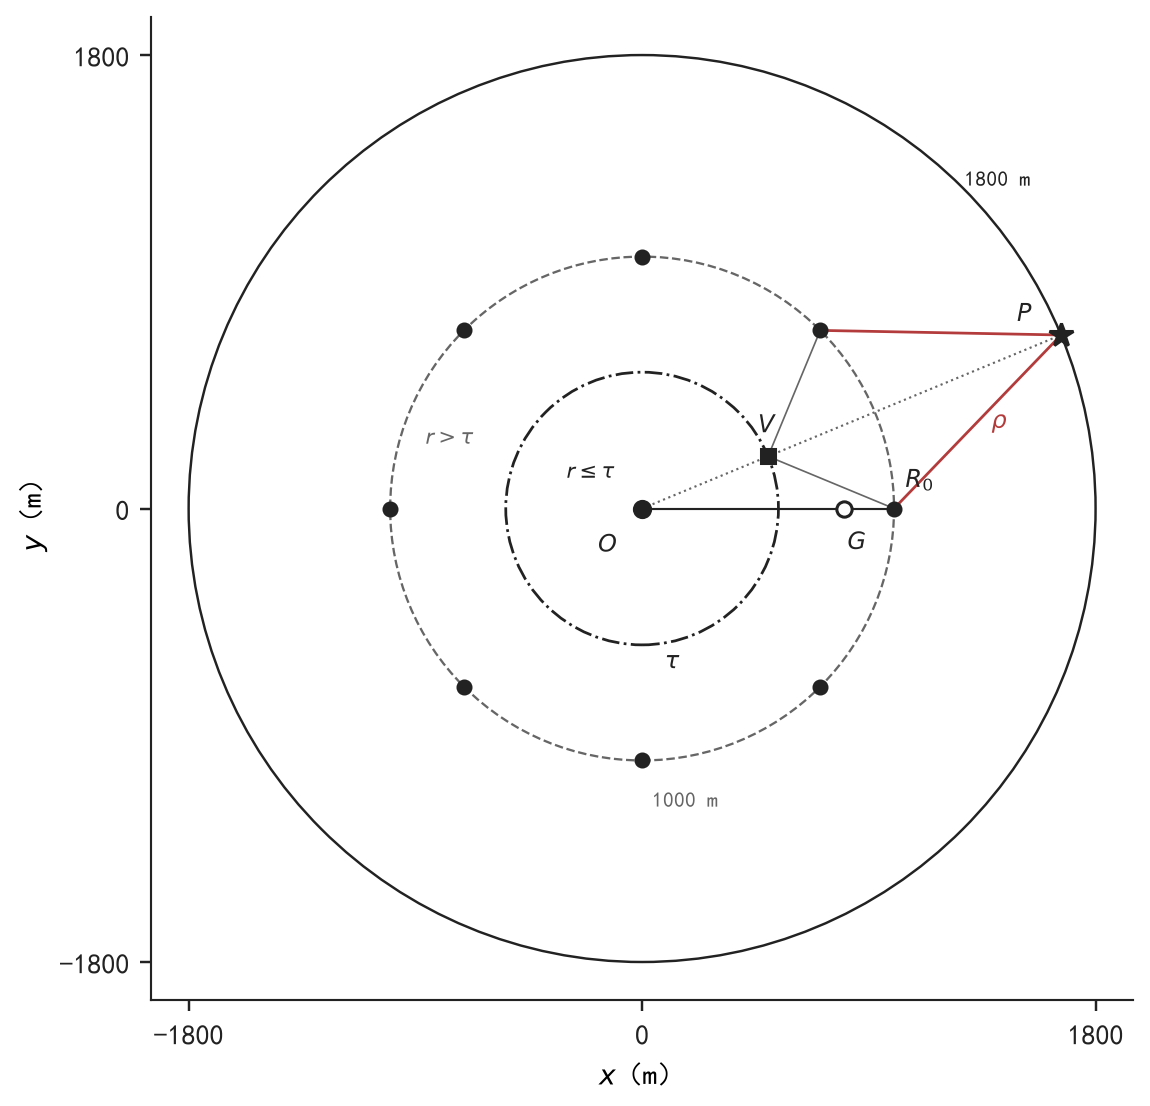
\includegraphics[width=0.59\textwidth]{figures/q3_nine_disk.png}
\caption{9点覆盖几何。实线圆为场地，虚线圆为环点所在圆，点划线半径$\tau$是证明分段界，不是圆形Voronoi胞腔。$V$是Voronoi顶点，$P$取到最远距离$\rho$。8环可用闭1000 m盘覆盖原点，但不能用半径$\rho$覆盖原点。}
\label{fig:ninedisk}
\end{figure}

\begin{table}[htbp]
\centering
\caption{问题三侦听点坐标（计算使用未取整坐标）}\label{tab:q3xy}
\begin{tabular}{crrl}\toprule
编号 & $x$/m & $y$/m & 角色\\\midrule
1 & 0 & 0 & 原点\\
2 & 1000 & 0 & 环$k=0$\\
3 & 707.1 & 707.1 & 环$k=1$\\
4 & 0 & 1000 & 环$k=2$\\
5 & $-707.1$ & 707.1 & 环$k=3$\\
6 & $-1000$ & 0 & 环$k=4$\\
7 & $-707.1$ & $-707.1$ & 环$k=5$\\
8 & 0 & $-1000$ & 环$k=6$\\
9 & 707.1 & $-707.1$ & 环$k=7$\\\bottomrule
\end{tabular}
\end{table}

\subsection{连续残留与可验证的保守剪枝}

设$\mathcal S$是实际\emph{完整且成功}扫描过当时所有静默频道的站点集合。定义
\begin{equation}
\mathrm{Res}_{\rm cont}(\mathcal S)=\mathbb A\setminus
\bigcup_{S\in\mathcal S}\overline{\mathbb D}(S,1000),\qquad
K_Q=\overline{\mathbb D}(Q,1000)\cap\mathbb A.\label{eq:rescont}
\end{equation}
任何尚未发现的源都属于该残留：若它距某发现站不超过1000 m，该站已经测量其频道，必然发现它。因而$K_Q$被已有发现站的1000 m盘覆盖时，可免去该覆盖义务。

\textbf{引理2（安全跳过）。}若$Q\in\mathbb A$且$K_Q\subseteq\bigcup_{S\in\mathcal S}\overline{\mathbb D}(S,1000)$，则$Q$不能听到尚未发现的源，即使该源的实际接收半径超过1000 m。

\textbf{证明。}假设$Q$能听到未发现源$G$，记$d=\|Q-G\|\le R_G$。若$d\le1000$，则$G\in K_Q$，与其未发现矛盾。若$d>1000$，在线段$QG$上取$\|Q-P\|=1000$。场地凸性保证$P\in K_Q$，故存在发现站$S$使$\|S-P\|\le1000$。于是$\|S-G\|\le1000+(d-1000)=d\le R_G$，该站本应听到$G$，仍矛盾。证毕。

在精确几何中，跳过等价于$\rho(\mathcal S,K_Q)=\max_{p\in K_Q}\min_{S\in\mathcal S}\|p-S\|\le1000$。用Voronoi顶点、边与边界圆交点、径向极值和透镜顶点枚举可以研究该最大值，但普通浮点枚举值不是自动带误差保证的上界。将判定阈值放宽为$1000+10^{-9}$同样不构成严格证书。

修订实现采用有理数矩形细分证书。将输入浮点数精确转换成其二进制有理数值，从包含$K_Q$的矩形开始，对每个矩形$B$执行：
\begin{enumerate}
\item 若$B$到某约束圆心的最小距离平方严格大于该圆半径平方，则$B$不与$K_Q$相交，可排除。
\item 若$B$四个角到某发现站的最大距离平方不超过$1000^2$，则整个矩形被该站覆盖，可认证。
\item 否则沿较长边对半细分；达到256个处理矩形的计算上限仍未结束，则返回“未认证”，保留侦听点。
\end{enumerate}
有限个已认证矩形覆盖所有可能与$K_Q$相交的区域，才能返回真。这里检查的是整块矩形的严格上界，不是有限点采样。若某约束圆盘本身已包含于一个发现站盘中，则用圆盘包含关系直接认证，特别覆盖扫描过的同中心盘。缓存使用原始坐标，不作六位小数舍入。证书不完备只会增加扫描，不会遗漏源。

原实现还使用内接正多边形裁剪场地和接收圆盘，可能切掉位于真实圆弧上的源，因此小多边形的包围圆不能直接当作真实可行集的清除证书。修订Q3的默认路径不使用该近似来决定清除；若进一步引入交会加速，应使用包含真实圆盘的外近似，并证明数值误差方向。

有限采样反例仍然成立。取$R_G=1000$，$G_\star=1800(\cos(\pi/24),\sin(\pi/24))$。其到$R_0$约819.023 m，到其余网点至少1176.405 m；八个边界角平分样本却可以全被其余网点覆盖。因此有限样本已空不能证明连续残留为空。反例明确取最小接收半径，不将“距其它站超过1000 m”误写成对所有$R_G$均不可听。

\subsection{距离上界收缩与有限步清除}

第一次得到\texttt{direction}时，只知道源位于该测向楔内且距离不超过1500 m。无须知道真实距离，也无须假设首次发现站是最近网点。

\textbf{引理3（半上界步进）。}在$S$测得单位示向度向量$u$，且已知$\|G-S\|\le R\le1500$。取
\begin{equation}
P=S+\frac R2u,\qquad \kappa=\sqrt{\frac54-\cos1^\circ}\approx0.5001523.
\label{eq:q3contract}
\end{equation}
则$\|G-P\|\le\kappa R$，且$\kappa R\le750.229<1000$，因此在$P$对该全向源测量必返回\texttt{direction}或\texttt{near}。

\textbf{证明。}记$r=\|G-S\|\in[0,R]$，误差$|\alpha|\le1^\circ$。余弦定理给出
\[
\|G-P\|^2=r^2+\frac{R^2}{4}-rR\cos\alpha
\le r^2+\frac{R^2}{4}-rR\cos1^\circ.
\]
右侧关于$r$凸，在$[0,R]$上的最大值位于端点，故不超过
$\max\{R^2/4,(5/4-\cos1^\circ)R^2\}=\kappa^2R^2$。
由于$R_G\ge1000$，新点仍可听。证毕。该论证逐步适用于任意允许误差序列，不依赖误差的概率分布。

代码使用更宽的收缩系数$\bar\kappa=0.501$，并采用递推
\begin{equation}
R_0=1500,\qquad R_{j+1}=0.501R_j+10^{-6}\quad (\mathrm m),
\label{eq:q3bound}
\end{equation}
同时向上取浮点相邻数，给坐标和三角函数运算留外向裕量。第$j+1$点仍取$S_j+(R_j/2)u_j$，不将坐标投影回场地圆盘；题目允许场地外检测。前六步若未返回\texttt{near}，在新点测量并更新示向度；第七步有$R_7<12<20$，直接清除，不再测量。若中途\texttt{near}则在该点清除。每源在首次发现后最多用六次测量加一次清除，共7次接口动作。

\begin{table}[htbp]
\centering
\caption{收缩清除的距离上界（按式\eqref{eq:q3bound}，向上显示）}
\label{tab:q3contraction}
\begin{tabular}{crl}\toprule
步数 & 上界/m & 动作\\\midrule
0 & 1500.000 & 已有首次示向度\\
1 & 751.501 & 测量；\texttt{near}则清除\\
2 & 376.502 & 测量；\texttt{near}则清除\\
3 & 188.628 & 测量；\texttt{near}则清除\\
4 & 94.503 & 测量；\texttt{near}则清除\\
5 & 47.346 & 测量；\texttt{near}则清除\\
6 & 23.721 & 测量；\texttt{near}则清除\\
7 & 11.884 & 直接清除\\\bottomrule
\end{tabular}
\end{table}

这一距离证书与问题一的包围圆证书一致：只要$G\in\Omega\subseteq\overline{\mathbb D}(C,20)$，在$C$清除就充分；不必先求出真实坐标或把多楔交压到20 m。相应地，若$G\in\Omega$且最小包围圆半径不超过1000 m，在其圆心再测对全向源可听。原先的轴上弦长$2r\sin(|\alpha|/2)$只适用于清除点轴向距离恰为未知真实距离$r$的构造，不是修订程序的步长规则，也不再承担可执行性证明。

\subsection{完整算法、动作上界与终止语义}

\begin{enumerate}
\item 成功\texttt{/enter}后，从返回值建立现实时间截止时刻；预留退出动作。先在原点测量所有静默频道，\texttt{near}就地清除，其余读数存储。
\item 剩余8个环点按当前位姿的开放TSP访问。每次取出一个环点；若其透镜有严格覆盖证书则跳过，否则完整扫描静默频道。仅在全部请求被接受、响应有效后，将该站加入发现集合。
\item 剩余环点为空、已发现16个不同频道，或静默频道为空时结束发现阶段。未知源数量不通过连续多次空扫来猜测。
\item 在已发现但未清除的频道中，选到其第一收缩点最近者，按引理3服务；完成后重新选择下一频道。无需先返回存储示向度的旧站，源位置固定保证旧读数仍有效。
\item 仅当发现已完成且所有已发现频道均收到成功清除响应时，输出\texttt{complete=true}。预算、超时、拒绝、无效响应、收缩点无信号或证书清除失败均输出明确未完成原因。
\end{enumerate}

\textbf{定理（Q3有限动作清除）。}在题设的全向、固定源、误差和接收半径条件下，若各请求在现实测试期限内正常接受并执行，则上述算法清除所有源。计入进入和退出，接口动作不超过
\begin{equation}
A\le1+9\cdot20+7N+1\le294<900.\label{eq:q3actions}
\end{equation}

\textbf{证明。}引理1保证每个源位于至少一个原始网点的1000 m盘内；引理2保证剪掉的透镜已由完整扫描覆盖。每轮处理并永久移除一个环点，最多8轮，不存在服务点反复插入造成的覆盖饥饿。若提前听满16个，由$N\le16$也已发现全部源。故发现阶段最多$9\cdot20$次测量。引理3保证每个已发现源最多7次服务动作后清除；发现时的\texttt{near}清除计入对应源的这7次额度。再计进入、退出各一次即得上界。证毕。

900是程序自设动作闸，并非原题常数。与只证明“正常结束时已发现”的命题相比，本定理给出模型内有限动作上界，因而默认动作闸不会截断有效轨迹。但动作数不等于现实用时，网络延迟、计算耗时、20分钟程序期限、25分钟窗口及技术异常仍可能使实际运行未完成；定理不把这些外部中断当作成功。

虚拟100小时上限也不会在模型内触发。覆盖段至多8次网点间移动，粗界16000 m。每条收缩链的相邻计划点总长小于1504 m，服务点到原点的距离不超过2504 m；从上一服务终点到下一第一收缩点的距离可粗界为4254 m。每源服务路程因此小于5758 m，全任务总路程小于110 km，移动与检测清除虚拟时间合计小于7小时。这只是保守可行性界，不是平均时间估计。开放TSP只精确优化当前覆盖站点的路程；未知源位置和后续服务仍使用启发式顺序。

\subsection{验证结果与历史演练的区分}

\begin{table}[htbp]
\centering
\caption{修订Q3的独立离线模型验证（非官方模拟器）}\label{tab:q3offline}
\begin{tabular}{lr}\toprule
量 & 结果\\\midrule
场景数 / 全清场景数 & 48 / 48\\
每场源数 & 10--16\\
动作次数范围（含进入退出） & 150--245\\
理论动作上界 & 294\\
总虚拟时间/总清除数（s/源） & 434.228\\
场均路程（m） & 22839.8\\
官方模拟器演练次数（修订代码） & 0\\\bottomrule
\end{tabular}
\end{table}


新代码的离线验证由\texttt{code/q3/offline\_validation.py}复现，随机种子从20260913起，共48个场景，源数循环取10至16。位置类型包含均匀圆盘、边界、聚簇及回归构型；误差类型包含恒定$+1^\circ$、恒定$-1^\circ$、零误差、随位置固定的有界误差和随位置固定的端点误差。回归构型含$G_\star$、原点近源及$(1400,0)$处接收半径1500 m的首次远距离发现。算法仅通过模拟客户端的测量与清除响应决策，测试器另用真值检查每一个收缩距离上界。

这些是按题设建立的独立离线模型测试，不是官方模拟器演练，不产生正式案例编码。完整结果和种子见\texttt{code/q3/offline\_results.json}。单元测试另覆盖亚微米和亚纳米剪枝反例、同心边界、细分预算耗尽、部分扫描被拒、动作预算、现实期限和证书清除失败；这些测试用于检查实现，不代替上述证明。

原包保留三次历史演练数据，见表\ref{tab:q3reh}。对应的是原覆盖骨架与射线启发式，原代码另存为\texttt{searcher\_legacy.py}。三次总虚拟时间除以总清除数的加权平均为
\[
\frac{3158.7139+3360.202868+3245.032067}{16+12+11}
\approx250.358\ \text{s/源}.
\]
该统计不等于三个案例均值的算术平均，也不是修订算法的速度。原包未提供足以重放这些案例的完整明文轨迹，故本次仅核对表格算术，不声称重新验证了这些官方演练结果。新旧场景不配对，不能据此宣称修订策略加速或减速。

\begin{table}[htbp]
\centering\scriptsize
\caption{原包历史Q3演练统计（旧启发式；不是修订代码成绩或正式测试）}\label{tab:q3reh}
\begin{tabular}{llrrrrr}\toprule
演练 & 案例编码 & 总数 & 清除 & 比例 & 动作 & 平均时间/s\\\midrule
1 & UUDJ-WJGP-NBRH-8V2N & 16 & 16 & 1.000 & 132 & 197.42\\
2 & XUXT-9646-NF9K-42J4 & 12 & 12 & 1.000 & 150 & 280.02\\
3 & 2GA6-9ADV-XD3E-AVMK & 11 & 11 & 1.000 & 160 & 295.00\\\bottomrule
\end{tabular}
\end{table}

原文另外列出24个旧同构场景全部清除、均值272.227 s/源、动作123至213的汇总；原包不含逐场景记录与对应测试器，本次不将其作为可复现的新验证结果。

\begin{figure}[htbp]
\centering
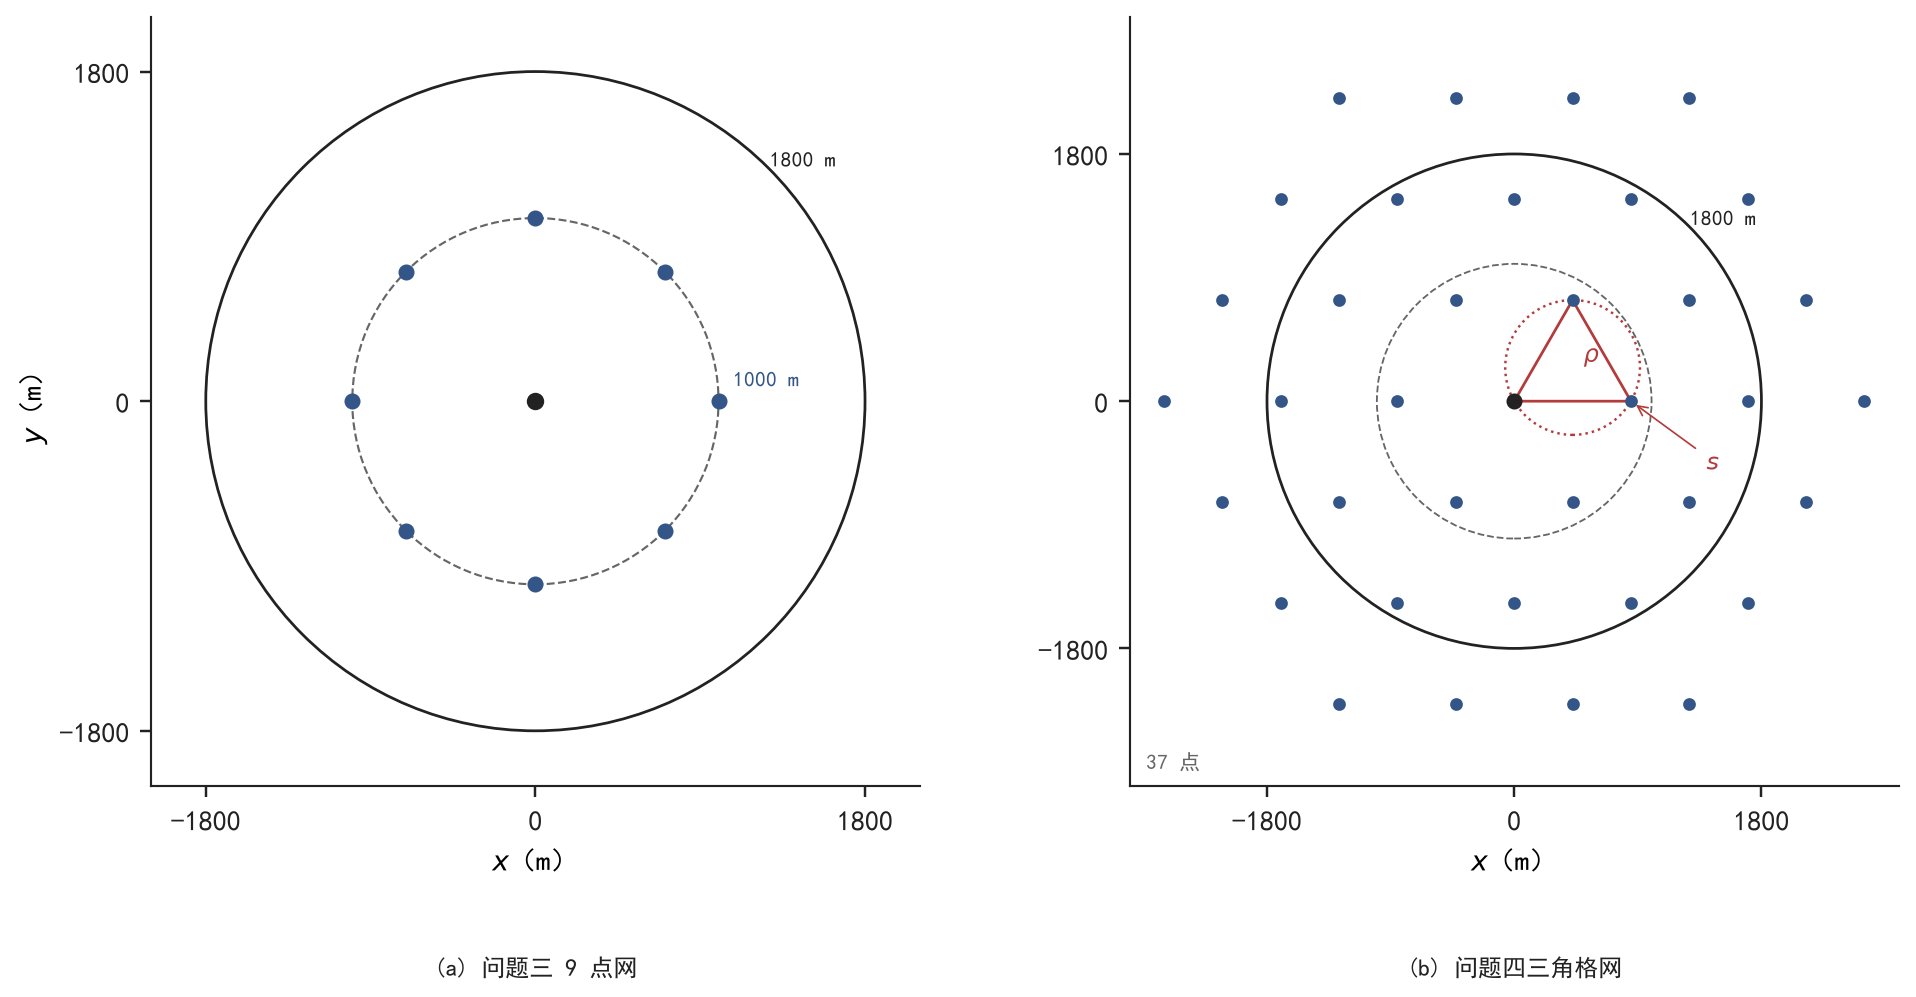
\includegraphics[width=0.94\textwidth]{figures/q34_scout_nets.png}
\caption{左：Q3原点加8环的侦听网；右：原文Q4三角格网。两问的方向假设不同，Q3收缩清除证明不能直接用于Q4。}\label{fig:scouts}
\end{figure}
\begin{figure}[htbp]
\centering
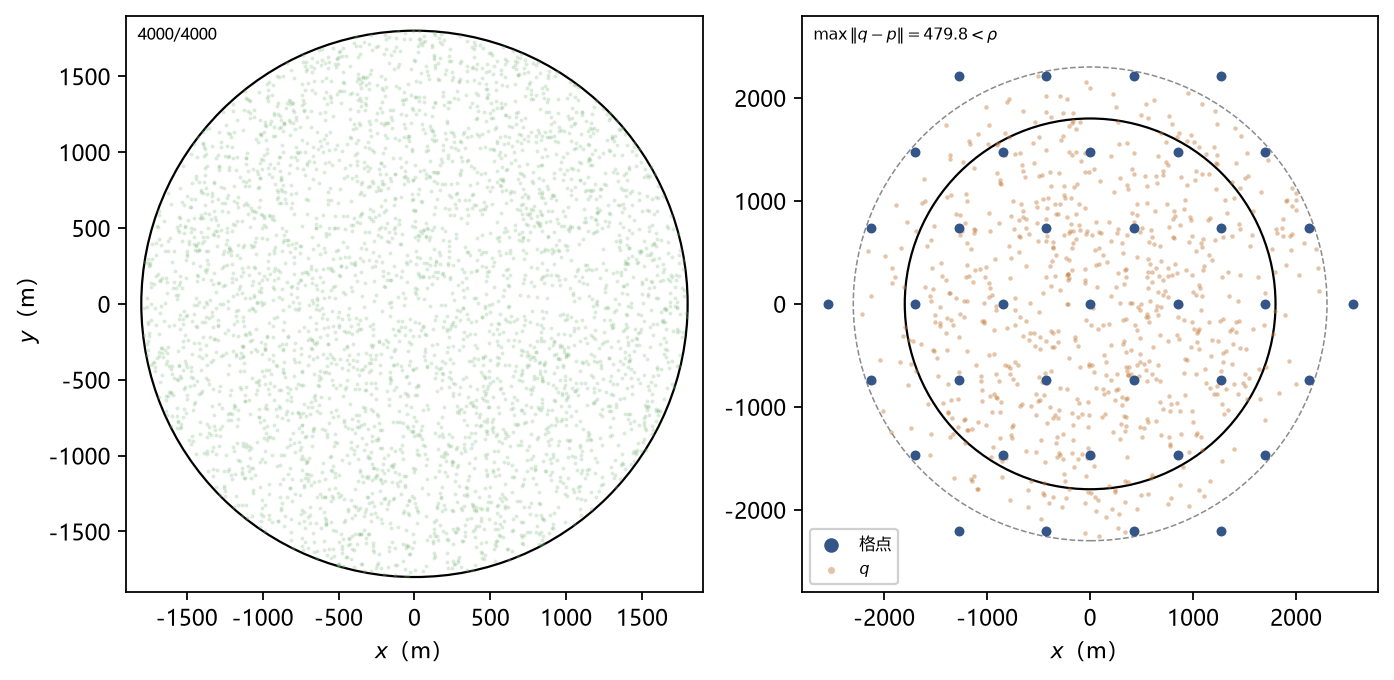
\includegraphics[width=0.94\textwidth]{figures/q34_coverage_scatter.png}
\caption{原包几何采样示意：左为Q3的4000个圆盘样本，右为Q4平移点与格点。采样图只作示意，Q3全称覆盖由引理1证明。}\label{fig:covmap}
\end{figure}

\subsection{正式测试与适用边界}

题目要求的三次正式测试尚无可核验数据。表\ref{tab:official3}保留题目表1的四个字段，测试序号写入案例编码栏；不得用旧演练或新离线结果补填。修订算法仍需在官方模拟器中演练，并导出三次正式日志，才能完成题目要求的实测交付。

\begin{table}[htbp]
\centering
\caption{问题三正式测试结果（待官方测试填写）}\label{tab:official3}
\begin{tabular}{lccc}\toprule
测试案例编码 & 清除干扰源个数 & 平均定位清除时间 & 程序运行时间\\\midrule
测试1：待测试 & --- & --- & ---\\
测试2：待测试 & --- & --- & ---\\
测试3：待测试 & --- & --- & ---\\\bottomrule
\end{tabular}
\end{table}

该算法提供有明确动作上界的可行解。它没有证明全任务时间最优；保守初始距离上界可能产生额外移动。今后的交会和D-最优加速应只减少已认证工作，或在有限预算内回退到本节的收缩步骤，不能重新引入无证书剪枝、以\texttt{no\_signal}猜测越源、或无上界的服务循环。所有结论限于Q3全向源，未将定向瓣的无信号解释成单纯超距。
\FloatBarrier


\section{问题四：定向源的三角格网发现与保扇形追逐}

\subsection{机理}

定向源在位置$G$、朝向$H$时，检测点$S$能收到信号当且仅当
\begin{equation}
\|S-G\|\le R_{\mathrm{eff}}\quad\text{且}\quad (S-G)\cdot u_H\ge 0,
\label{eq:dir}
\end{equation}
其中$u_H=(\cos H,\sin H)$。从$G$看，闭瓣是过$G$且法向为$u_H$的闭半平面。如图\ref{fig:sector}所示，有效覆盖是以$G$为顶点、朝向两侧各90度的闭扇形。最小接收半径只约束距离因子：落在背面的检测点即使$\|S-G\|\le 1000$ m也给出\texttt{no\_signal}。因此单次无信号不能把该频道标死，问题三的全向收缩清除证明也不能搬到本问。光学清除只依赖距离，问题一的圆心规则仍然充分。

发现层需要的是对一切$G\in\mathbb{D}(0,1800)$与一切朝向$u$的可听证书，而不是抽样覆盖率。把侦听点放到沿发射方向平移$a=500$ m的点$q=G+au$的$\rho$-邻域内，则
\begin{equation}
\|p-G\|\le a+\rho,\qquad (p-G)\cdot u\ge a-\rho.
\label{eq:aplus}
\end{equation}
存在这样的$a$当且仅当格网覆盖半径$\rho<500$ m。如图\ref{fig:dirlisten}所示，源在$G=(200,0)$、朝向正东时，平移点$q=(700,0)$，格点$p=(850,0)$落入以$q$为心、半径$\rho$的闭圆盘，并落在前向瓣内；背面格点听不到该朝向。如图\ref{fig:spoke}所示，同一构型沿轴线把$a$与$\rho$分开画出：$G$到$q$为平移量，$q$到$p$不超过覆盖半径。

\begin{figure}[htbp]
\centering
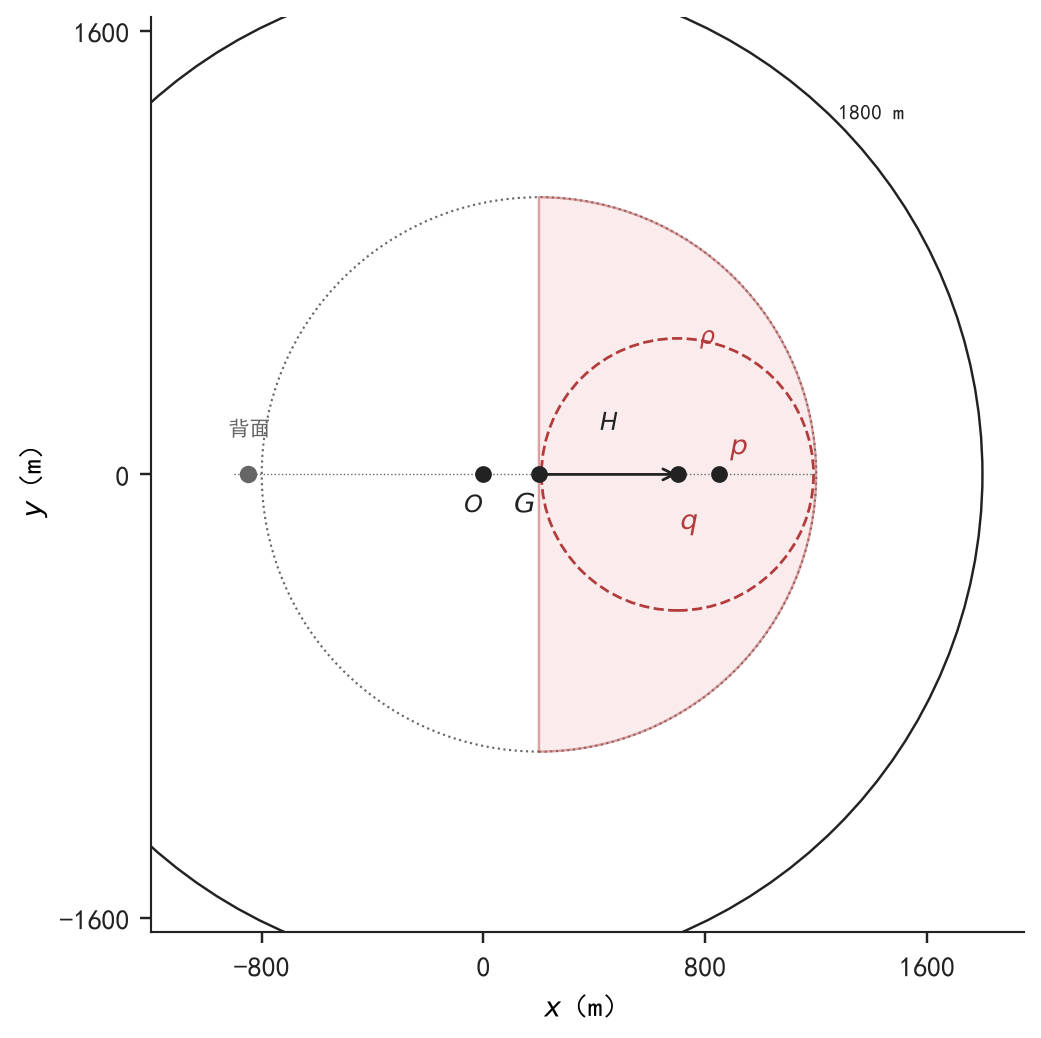
\includegraphics[width=0.72\textwidth]{figures/directional_listen.png}
\caption{定向源的可听半平面。$G$在$(200,0)$ m，朝向$H$指向正东；$q=G+500u$，$p$为覆盖$q$的格点，虚线圆半径为$\rho$；左侧灰点落在背面。}
\label{fig:dirlisten}
\end{figure}

\begin{figure}[htbp]
\centering
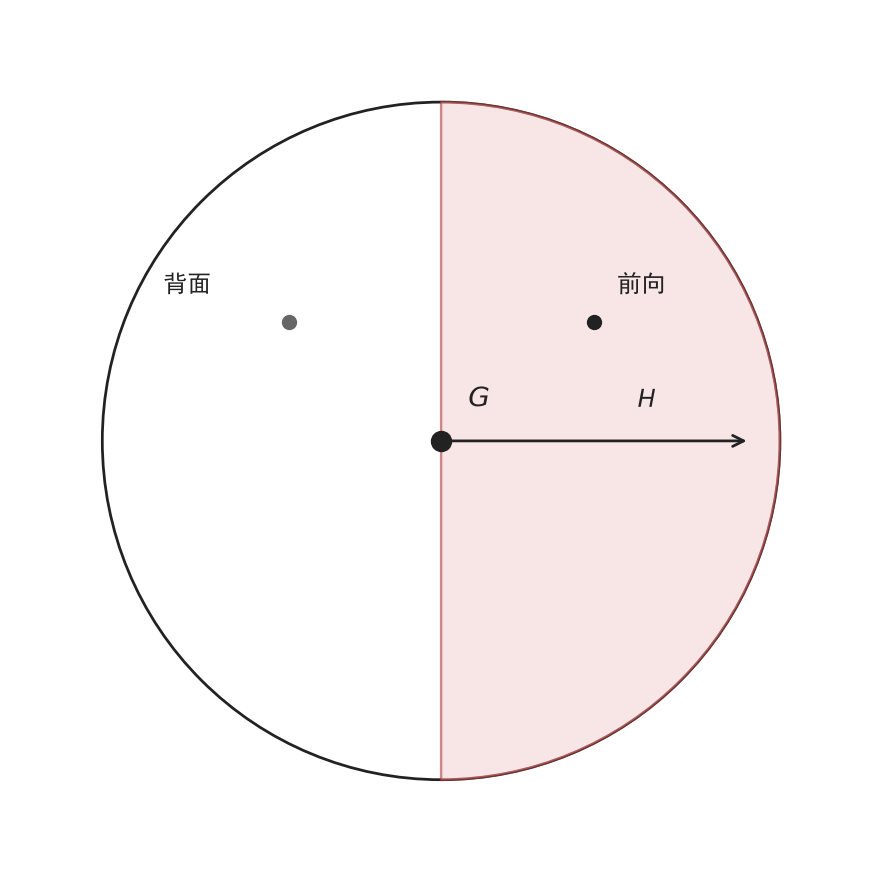
\includegraphics[width=0.55\textwidth]{figures/q4_directional_sector.png}
\caption{定向源的有效覆盖为朝向两侧各90度的闭扇形。$G$在圆心，$H$指向前向瓣。}
\label{fig:sector}
\end{figure}

\begin{figure}[htbp]
\centering
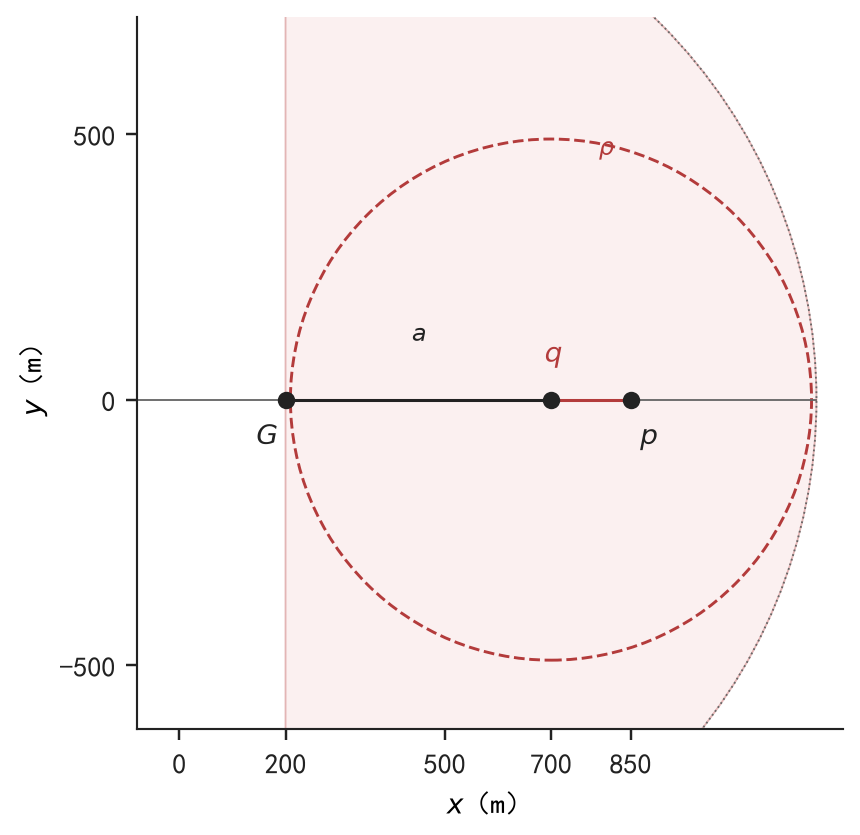
\includegraphics[width=0.92\textwidth]{figures/q4_silent_spoke.png}
\caption{发现引理的轴向剖面：$G$在200 m，$q$在700 m，$p$在850 m；虚线圆是覆盖半径$\rho$，阴影为前向瓣。}
\label{fig:spoke}
\end{figure}

\subsection{模型}

侦听网取由向量$(s,0)$与$(s/2,\,s\sqrt{3}/2)$生成的三角格点，并截断到$\mathbb{D}(0,1800+a+\rho)$，见表\ref{tab:q4pts}。其基本形式为：格点
\[
p_{jk}=j\,(s,0)+k\bigl(s/2,\,s\sqrt{3}/2\bigr),\qquad j,k\in\mathbb{Z},
\]
满足$\|p_{jk}\|\le 1800+a+\rho$的全部点。边长取$s=850$ m，平移量取$a=500$ m，有限集共37点。如图\ref{fig:scouts}右幅所示，原点附近的等边三角形外接圆半径即为覆盖半径。内点与外点一视同仁：静默频道在剩余格点上扫描，已有示向度的频道不再为它走完格网。每次在剩余格点中取距当前位置最近者访问；追逐结束后下一站重新按最近剩余选取。点位清单见附录表\ref{tab:q4visit}，该表不是固定走环。混编覆盖循环另设动作闸$A_{\max}=900$。格网引理给出的是某一格点可听；走完剩余格点是证书动作。预算用尽、超时或异常时尚未访问的格点可以仍对某个定向源可听，该残差与问题三检测定理的非正常结束残差同构。追逐层已经把证书成立与预算用尽写成并列。

\textbf{引理（平移量存在当且仅当$\rho<500$）。}设$R_{\mathrm{eff}}=1000$ m。若格网覆盖半径为$\rho$，则存在$a>0$使$a+\rho<1000$且$a-\rho>0$，当且仅当$\rho<500$。充分性：取$a=500$。必要性：两式相加得$2a<1000$，相减得$2\rho<1000$。

\textbf{引理（三角格网覆盖半径）。}上述格点的Voronoi胞腔是对边距为$s$的正六边形，覆盖半径等于等边三角形外接半径
\begin{equation}
\rho=\frac{s}{\sqrt{3}}.
\label{eq:q4rho}
\end{equation}
$s=850$ m时$\rho\approx 490.75$ m，等边三角形外心到三顶点的距离与之相等。

\textbf{引理（有限圆盘截断仍覆盖$q$-盘）。}设$G\in\mathbb{D}(0,1800)$，$q=G+au$，则$q\in\mathbb{D}(0,1800+a)$。若$p$满足$\|p-q\|\le\rho$，则$\|p\|\le 1800+a+\rho$。因此把格点限制在该闭圆盘内，仍包含无限格网上覆盖$q$的那一个点。$s=850$、$a=500$时该有限集为37点。

\textbf{引理（格点检测，定向瓣）。}假设$R_{\mathrm{eff}}=1000$ m，$\rho<500$，$a=500$，$p$为$q=G+au$的覆盖格点。则$\|p-G\|\le a+\rho<1000$，$(p-G)\cdot u\ge a-\rho>0$，故$p$落在开瓣与开距离盘内，检测方程成立。$s=850$时$a+\rho\approx 990.75$ m，$a-\rho\approx 9.25$ m。

\textbf{命题（$s=900$不合格）。}$s=900$ m时$\rho=900/\sqrt{3}\approx 519.62>500$，不存在合格平移量。间距上界是
\begin{equation}
s<500\sqrt{3}\approx 866.03\,\mathrm{m}.
\label{eq:smax}
\end{equation}
等号使$\rho=500$，距离和恰为1000 m，开距离盘条件不成立，故交付间距必须严格小于该上界。

\textbf{引理（光学方格清除）。}边长25 m的闭正方形，格心到顶点距离$25/\sqrt{2}\approx 17.68<20$。故若$G$落在该格内，在格心\texttt{/clear}必中。当$\Omega\subseteq\overline{\mathbb{D}}(C,R_{\mathrm{sec}})$且$R_{\mathrm{sec}}\le 80$ m时，在该盘上铺此方格是清除证书，不是抽样。如图\ref{fig:optical}所示，虚线为清除半径20 m，实线为启用该证书的80 m盘。

\textbf{引理（精确示向度下沿测向线越过源）。}假设第一站$S$落在开瓣$\{X:(X-G)\cdot u_H>0\}$内，且第二站沿精确方位$u=(G-S)/\|G-S\|$行走。则当路程$t<\|G-S\|$时仍在开瓣内；当且仅当$t>\|G-S\|$时落入互补开半平面，该站为\texttt{no\_signal}。若示向度含$\pm 1^\circ$误差，行走线不必过$G$，结论不必成立。

\textbf{引理（侧向位移，带假设）。}记$v$为测得示向度的单位左转法向，$P(t)=S+tv$。$P(t)$对一切实数$t$都留在闭瓣内，当且仅当$v\perp H$。否则逃逸阈值为
\[
|t|=\frac{(S-G)\cdot u_H}{|v\cdot u_H|},
\]
更大的$|t|$离开闭瓣。因此侧向$S+tv$并不总是留在扇形内；实现里对\texttt{no\_signal}立即换侧，正是因为$t$与$H$的相对方位事先未知。保扇形$(r,t)$列表是时间启发式，不是瓣的覆盖集。

追逐采用保扇形追逐（sector-preserving chase）。其基本形式为：在已测到示向度的站$S$上取
\[
S'=S+r\,u_{\theta}+t\,v_{\theta},
\]
其中$r$取短沿迹、$t$取侧向；若$S'$返回\texttt{no\_signal}，立即翻转$180^\circ$侧向假设，而不是沿用问题二的$(800,700)$ m长跨步。如图\ref{fig:secchase}所示，源朝向$H$指向$S_1$所在半平面：左幅沿示向度越过$G$的第二站落入无阴影的背面；右幅取$(r,t)=(60,500)$ m，第二站留在同一闭扇形内。两站示向度差小于$8^\circ$时视为共线，改取纯侧向站拉开交角。清除半径20 m与朝向无关。问题二的解析交付点$(800,700)$ m不进入本问的定向第二站，也不作为问题三全向追逐的默认第二站。

场地点的内点计划为
\[
(r,t)\in\bigl\{(150,\pm 400),\,(60,\pm 500),\,(250,\pm 200),\,(100,0)\bigr\}\,\mathrm{m};
\]
其中前两项$(150,\pm 400)$ m的模长均为
\begin{equation}
\sqrt{150^2+400^2}\approx 427.2\,\mathrm{m}.
\label{eq:q4step}
\end{equation}
外点第一站则取更贴边的
\[
(r,t)\in\bigl\{(80,\pm 450),\,(0,\pm 550),\,(160,\pm 300),\,(250,0)\bigr\}\,\mathrm{m}.
\]
共线侧向取$r=0$、$t\in\{\pm 500,\pm 350,\pm 700\}$ m。问题二交付点的站距为$\sqrt{800^2+700^2}\approx 1063.0$ m，与式\eqref{eq:q4step}不是同一跨步。

混编追逐写成有限次循环，上限取10次，分款见表\ref{tab:q4chase}。每一次循环按当前示向度条数分支。定位多边形的半径判定与问题三共用同一套规则，定向瓣只改变圆心再测的可听含义。

\begin{enumerate}
\item 仅一站示向度：按上列$(r,t)$表作保扇形第二站，\texttt{no\_signal}立即换侧。若该表推进了新的测向记录，进入下一次循环。若全部候选都未能推进，沿测得示向度按路程
\[
\{120,250,400,600,850,1100\}\,\mathrm{m}
\]
前进：返回\texttt{near}则清除；返回\texttt{direction}则更新最后命中点并继续前进；返回\texttt{no\_signal}则先对最后命中点与当前点的中点执行\texttt{/clear}，失败后再清最后命中点。该沿示向度路程是瓣内最后手段，不是一站之后的默认第二站。
\item 两站示向度差小于$8^\circ$：改纯侧向站。若侧向推进了交角不小于$8^\circ$的新示向度，进入下一次循环；若未能推进，同样进入上述沿示向度路程。
\item 两站非共线：先做多边形清除判定。证书半径仍是$R_{\mathrm{sec}}\le 20$ m或对径圆且$D/2\le 20$ m。若$20\,\mathrm{m}<R_{\mathrm{sec}}\le 1000$ m，仍在最小包围圆圆心测量：返回\texttt{near}则清除；返回\texttt{direction}则把新楔并入$\Omega$并进入下一次循环。圆心再测对定向瓣不再是“必听到”：源可能落在背面。若圆心返回\texttt{no\_signal}且$R_{\mathrm{sec}}\le 80$ m，先在圆心强制\texttt{/clear}，失败后再用18 m六邻点
\[
C+18\bigl(\cos\tfrac{k\pi}{3},\sin\tfrac{k\pi}{3}\bigr),\qquad k=0,\ldots,5
\]
补清除；$18+20=38$ m只覆盖近心邻域，不能代替更新$\Omega$，也覆盖不了半径80 m的不确定盘。六邻点之后若仍未清除，才把判定标成开放。若$R_{\mathrm{sec}}>1000$ m，圆心再测不执行，判定直接为开放。判定开放后，对最后一站再跑保扇形$(r,t)$表，把新楔并入$\Omega$。这是短沿迹尚未把$\Omega$压进证书半径时的主局部化步。仅当这次保扇形也未能推进时，才进入沿示向度路程。
\end{enumerate}

仅当循环用尽且频道仍未清除时，先在当时最小包围圆圆心强制执行一次\texttt{/clear}；若$R_{\mathrm{sec}}\le 80$ m仍未清除，则铺25 m光学方格；光学方格之后若仍未清除，再沿最后一站示向度走上述$\{120,\ldots,1100\}$ m路程。圆心强制清除在$R_{\mathrm{sec}}>20$ m时不是覆盖证书。时间启发式失败时回退到证书动作：静默频道仍在则继续走剩余格点；未达$R_{\mathrm{sec}}\le 20$ m则继续保扇形测站直到证书成立或预算用尽。

\begin{table}[htbp]
\centering
\caption{问题四混编追逐：分款与局部化循环}
\label{tab:q4chase}
\begin{tabular}{>{\raggedright\arraybackslash}p{0.46\textwidth}>{\raggedright\arraybackslash}p{0.46\textwidth}}
\toprule
条件 & 动作 \\
\midrule
一站示向度 & 保扇形短沿迹加侧向；内点首项$(150,\pm 400)$ m，模长$427.2$ m；\texttt{no\_signal}立即换侧 \\
一站保扇形已推进 & 进入下一次循环 \\
一站保扇形未推进 & 沿示向度$\{120,\ldots,1100\}$ m（瓣内最后手段） \\
两站示向度差小于$8^\circ$ & 纯侧向站拉开交角 \\
共线侧向未推进 & 沿示向度路程 \\
两站非共线且$R_{\mathrm{sec}}\le 20$ m，或对径圆覆盖且$D/2\le 20$ m & 在该圆心\texttt{/clear}（清除证书） \\
$20\,\mathrm{m}<R_{\mathrm{sec}}\le 1000$ m & 仍在最小包围圆圆心测量 \\
圆心再测返回\texttt{near} & 在圆心清除 \\
圆心再测返回\texttt{direction} & 新楔并入$\Omega$，重入循环 \\
圆心再测返回\texttt{no\_signal}且$R_{\mathrm{sec}}\le 80$ m & 先圆心强制\texttt{/clear}，再18 m六邻点，然后才把判定标成开放 \\
多边形判定仍开放（含$R_{\mathrm{sec}}>1000$ m，或再测与六邻点仍未清除） & 对最后一站再跑保扇形（主局部化步） \\
保扇形仍未推进 & 沿示向度路程 \\
循环10次用尽仍未清除 & 圆心强制\texttt{/clear}；$R_{\mathrm{sec}}\le 80$ m时铺光学方格；其后仍走沿示向度路程 \\
\bottomrule
\end{tabular}
\end{table}

\begin{table}[htbp]
\centering
\caption{问题四三角格网的构成}
\label{tab:q4pts}
\begin{tabular}{lccc}
\toprule
量 & 取值 & 个数 & 说明 \\
\midrule
格点间距 $s$ / m & 850 & --- & 严格小于$500\sqrt{3}$ \\
平移量 $a$ / m & 500 & --- & $\rho<500$时的可行取值 \\
覆盖半径 $\rho$ / m & 490.75 & --- & $s/\sqrt{3}$ \\
有限格点 & --- & 37 & 截断到$\mathbb{D}(0,1800+a+\rho)$ \\
光学方格边长 / m & 25 & --- & 格心外接半径$17.68<20$ \\
\bottomrule
\end{tabular}
\end{table}

\begin{figure}[htbp]
\centering
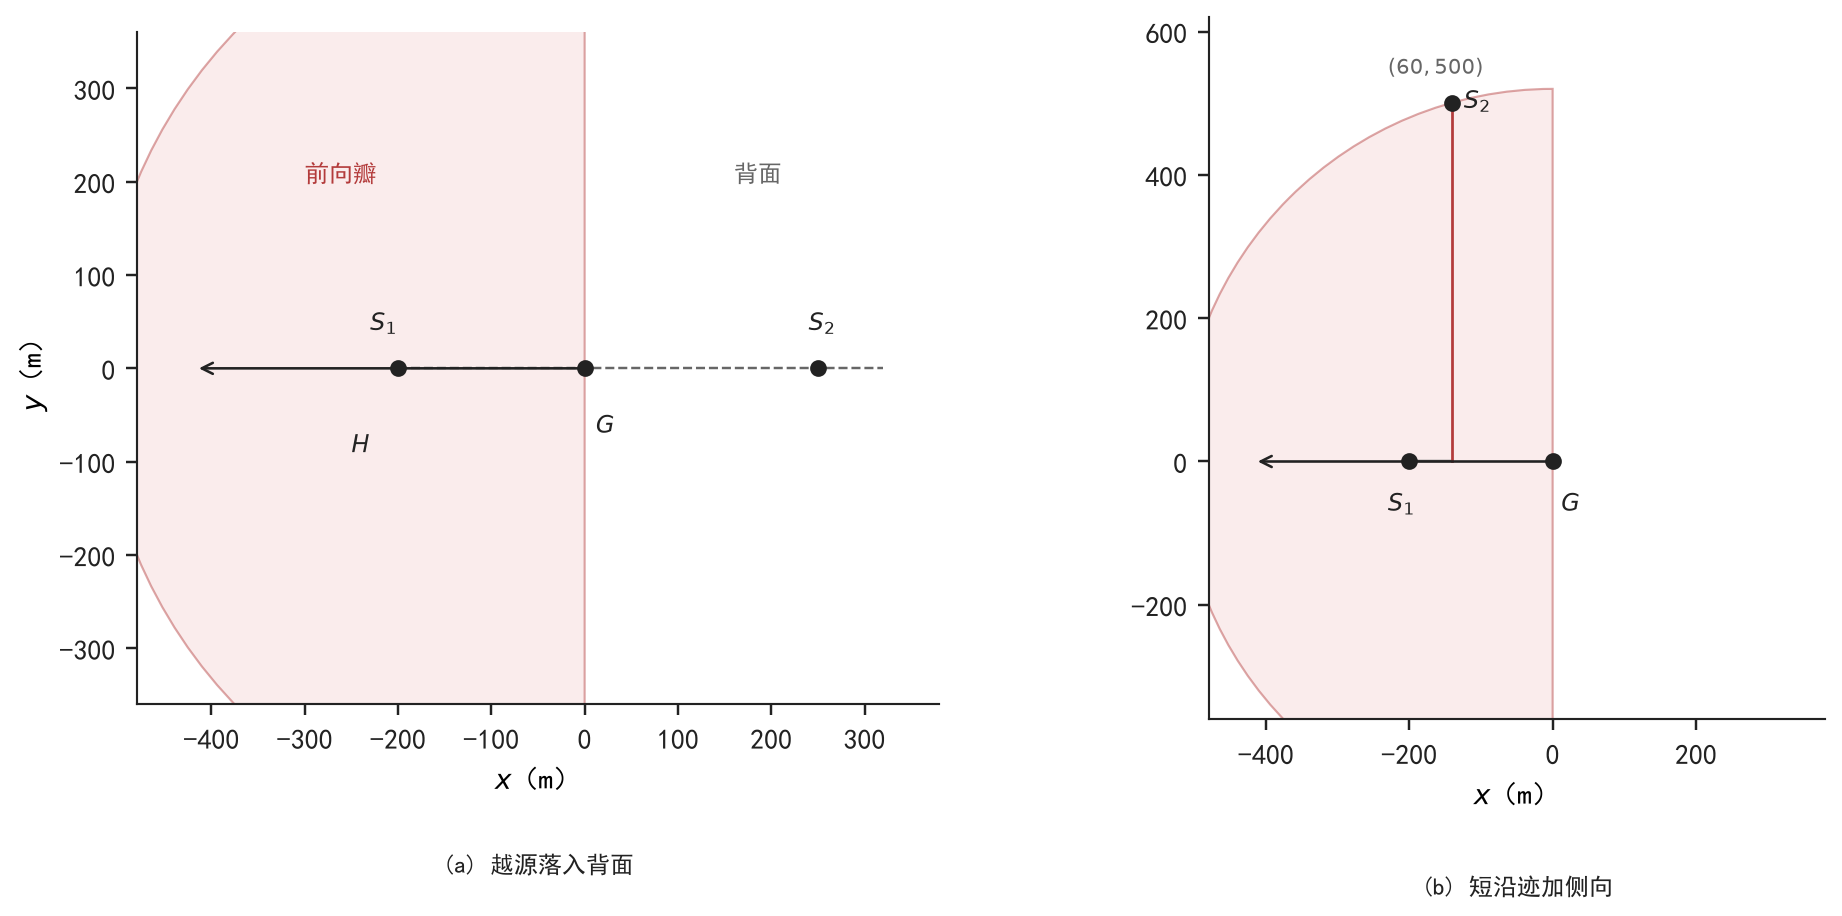
\includegraphics[width=0.98\textwidth]{figures/q4_sector_chase.png}
\caption{保扇形第二站。朝向$H$指向$S_1$所在半平面。左：沿示向度越过源，落入背面；右：$(r,t)=(60,500)$ m留在同一闭扇形内。}
\label{fig:secchase}
\end{figure}

\begin{figure}[htbp]
\centering
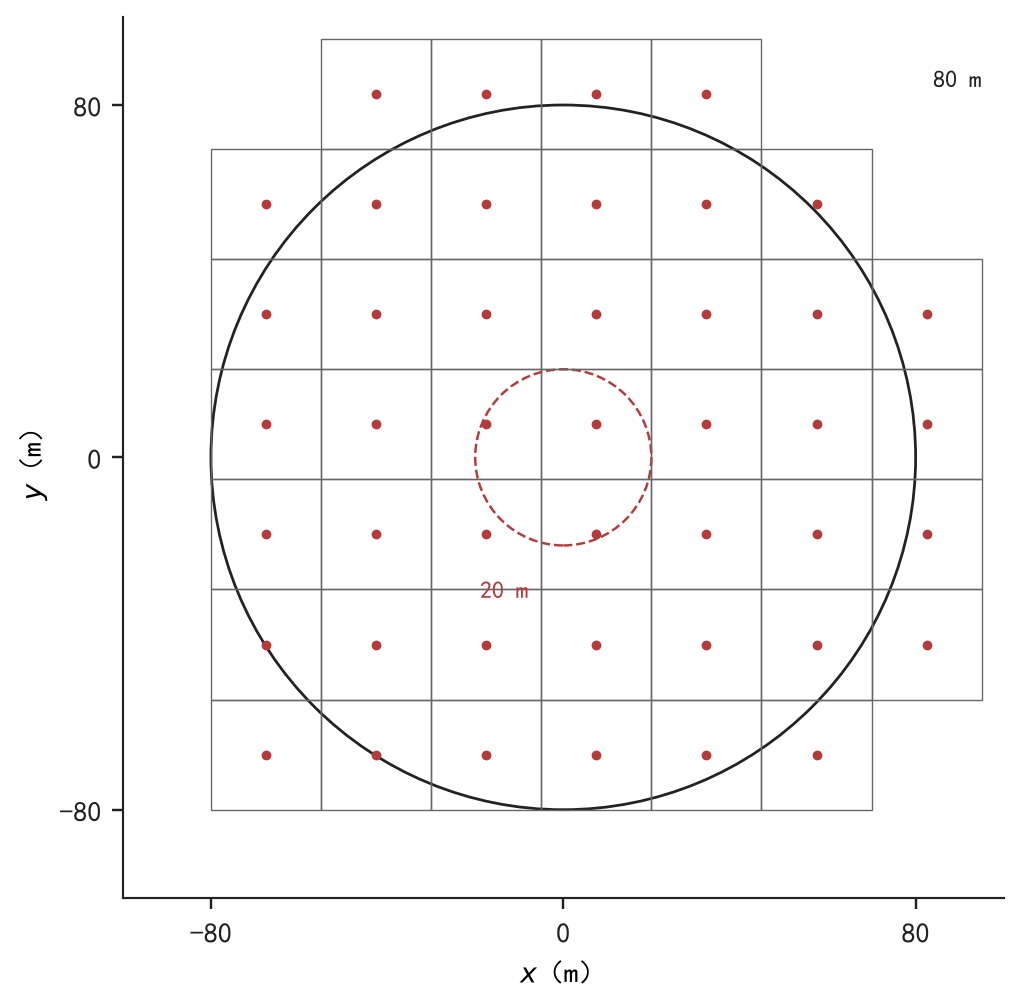
\includegraphics[width=0.55\textwidth]{figures/q4_optical_grid.png}
\caption{光学方格清除证书：边长25 m的闭正方形外接半径约17.68 m，小于清除半径20 m；实线盘半径80 m是启用该证书的限度。}
\label{fig:optical}
\end{figure}

\subsection{估计与检验}

发现证书是式\eqref{eq:q4rho}--\eqref{eq:smax}的闭式界，不是覆盖率抽样。$s=850$ m时$\rho\approx 490.75$ m$<500$ m，$a+\rho\approx 990.75$ m$<1000$ m，$a-\rho\approx 9.25$ m$>0$。$s=900$ m时$\rho\approx 519.62$ m，不存在合格$a$。极坐标$\times$朝向网格$n_r=8$、$n_{\theta}=16$、$n_H=12$共1536个样本上，全部被某一格点听到；该网格是核对，不是覆盖模型。光学方格外接半径$17.68$ m$<20$ m，覆盖布尔值为1。

演练窗口给出两组独立案例，策略参数见表\ref{tab:q4policy}。本问交付的侦听网是边长$850$ m的三角格点$37$个，追逐内点首项为$(r,t)=(150,\pm 400)$ m，模长约$427.2$ m。该策略上的三次独立案例编码为JXCC-FPAB-8G8W-38NV、YQTQ-FT7R-JXAJ-VSYX、JQ6W-RHH2-2W69-K9Z9，三次连续全部清除；含定向源时，本问交付策略的演练实现以该列为准。窗口另有三次独立案例，编码为XU7K-FB9B-7CBC-V9JH、7GX8-6986-P9P4-4JZG、A69F-C2FE-ZDNT-JMGF。该组日志中的侦听点含原点以及半径$900$ m与$2100$ m的同辐条八点，合计$17$点；第二站取问题二交付点$(800,700)$ m，相邻新站距离$\sqrt{800^2+700^2}\approx 1063.0$ m。按式\eqref{eq:q4rho}的$37$点格网与式\eqref{eq:q4step}的保扇形复现路径，侦听半径应落在格点模长上、第二站模长应为$427.2$ m，因而不能复现该组$338/480/299$次动作、$900$ m侦听与$(800,700)$ m长跨步。窗口三次只作为另一套侦听与追逐规则的窗口记录展示，不是本问交付策略的清除比例点估计。两组都不是正式测试，也不能当作同一策略的前后对照。正式测试表与问题三同格式，不填入任一演练行。

\subsection{结果}

由表\ref{tab:q4cov}可知，三角格网共37点，间距850 m，覆盖半径$\rho\approx 490.75$ m，小于500 m；平移量500 m时距离和约990.75 m，半平面余量约9.25 m。由表\ref{tab:q4cert}可知，间距上界约866.03 m，交付间距850 m严格小于该上界；间距900 m的覆盖半径约519.62 m，合格平移量为0。如图\ref{fig:scouts}所示，右幅把37个格点画在场地圆盘内外，红色等边三角形的外接圆即覆盖半径。如图\ref{fig:covmap}所示，左幅4000个均匀圆盘样本在9点网上全部距离可听，是问题三闭式界的核对；右幅800个$q=G+500u$样本相对37格点的最近距离最大为479.8 m，小于$\rho$，是格网覆盖引理的核对而不是定理。如图\ref{fig:dirlisten}与图\ref{fig:spoke}所示，前向瓣内的格点$p$同时满足距离与半平面，背面格点听不到。

\begin{table}[htbp]
\centering
\caption{问题四三角格网发现证书}
\label{tab:q4cov}
\begin{tabular}{lr}
\toprule
量 & 取值 \\
\midrule
侦听点个数 & 37 \\
间距 $s$ / m & 850 \\
平移量 $a$ / m & 500 \\
覆盖半径 $\rho$ / m & 490.7477288111819 \\
$a+\rho$ / m & 990.7477288111819 \\
$a-\rho$ / m & 9.2522711888181 \\
距离条件 $a+\rho<1000$ & 1 \\
半平面条件 $a-\rho>0$ & 1 \\
存在合格平移量 & 1 \\
\bottomrule
\end{tabular}
\end{table}

\begin{table}[htbp]
\centering
\caption{问题四间距上界、不合格间距与光学证书}
\label{tab:q4cert}
\begin{tabular}{lr}
\toprule
量 & 取值 \\
\midrule
间距上界 $500\sqrt{3}$ / m & 866.0254037844386 \\
交付间距是否小于上界 & 1 \\
$s=900$ m覆盖半径 / m & 519.6152422706632 \\
$s=900$ m存在合格平移量 & 0 \\
等边三角形外接半径 / m & 490.7477288111819 \\
极坐标$\times$朝向网格点数 & 1536 \\
网格全部可听 & 1 \\
该网格是否覆盖定理 & 0 \\
光学方格边长 / m & 25 \\
光学格心外接半径 / m & 17.677669529663685 \\
光学方格覆盖 & 1 \\
\bottomrule
\end{tabular}
\end{table}

\begin{table}[htbp]
\centering
\caption{问题四两组演练的策略参数。窗口三次侦听半径与第二站来自行为日志；格网三次与正文三角格网加保扇形一致。}
\label{tab:q4policy}
\scriptsize
\begin{tabular}{lcccc}
\toprule
组别 & 侦听网 & 点数 & 第二站 & 站距 / m \\
\midrule
窗口三次 & 原点加$900$ m与$2100$ m同辐条八点 & 17 & $(800,700)$ m & 1063.0 \\
格网三次 & 边长$850$ m三角格点 & 37 & 内点首项$(150,\pm 400)$ m & 427.2 \\
\bottomrule
\end{tabular}
\end{table}

由表\ref{tab:q4full}可知，本文三角格网加保扇形在三个独立案例上的干扰源总数为10、12、12，全向源分别占0、8、10，定向源分别占10、4、2，清除个数与总数相同，比例均为1。动作次数为507、438、415，平均定位清除时间为1502.4 s、1303.7 s、1205.9 s，虚拟时间为15024 s、15644 s、14470 s。如图\ref{fig:q4full}所示，真实个数与清除个数三次重合。该组是边长$850$ m的$37$点格网与保扇形短沿迹在另外三个独立案例上的连续全部清除，不得抄入正式测试表。

\begin{table}[htbp]
\centering
\caption{问题四三角格网加保扇形的连续三次演练（全部清除）}
\label{tab:q4full}
\scriptsize
\begin{tabular}{llrrrrrr}
\toprule
演练 & 案例编码 & 总数 & 全向 & 定向 & 清除 & 比例 & 动作 \\
\midrule
1 & JXCC-FPAB-8G8W-38NV & 10 & 0 & 10 & 10 & 1.000 & 507 \\
2 & YQTQ-FT7R-JXAJ-VSYX & 12 & 8 & 4 & 12 & 1.000 & 438 \\
3 & JQ6W-RHH2-2W69-K9Z9 & 12 & 10 & 2 & 12 & 1.000 & 415 \\
\bottomrule
\end{tabular}
\end{table}

\begin{table}[htbp]
\centering
\caption{问题四三角格网加保扇形三次演练的时间统计}
\label{tab:q4fullt}
\begin{tabular}{lrrr}
\toprule
演练 & 虚拟时间 / s & 平均定位清除时间 / s & 动作次数 \\
\midrule
1 & 15023.990 & 1502.399 & 507 \\
2 & 15644.485 & 1303.707 & 438 \\
3 & 14470.475 & 1205.873 & 415 \\
\bottomrule
\end{tabular}
\end{table}

\begin{figure}[htbp]
\centering
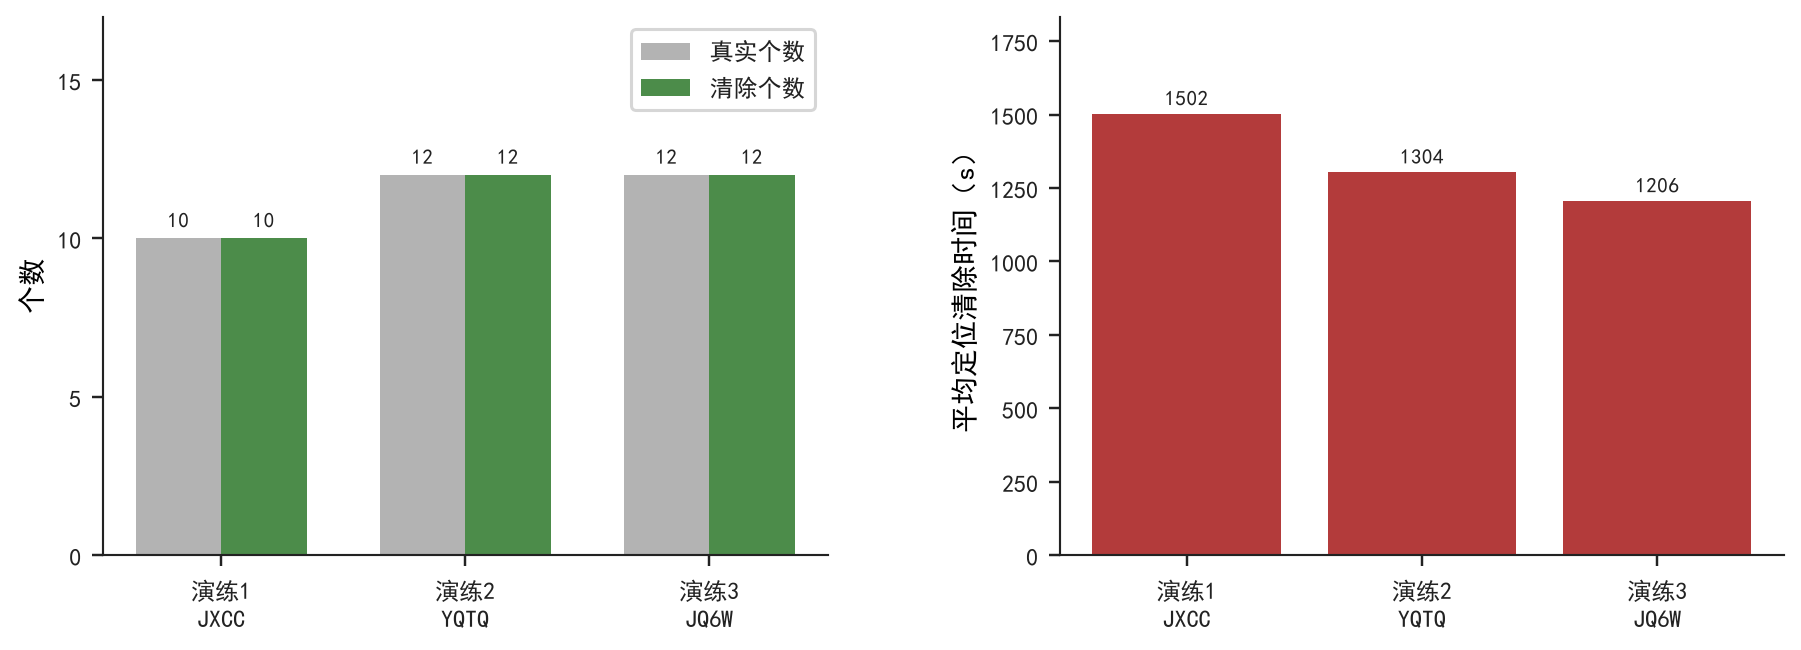
\includegraphics[width=0.98\textwidth]{figures/q4_fullclear_bars.png}
\caption{问题四三角格网加保扇形的连续三次演练：真实个数与清除个数重合；右幅为平均定位清除时间。}
\label{fig:q4full}
\end{figure}

方法一即上述三角格网加保扇形。方法二把37点格网发现证书从时间层拿掉：内圈用问题三的9点网对静默频道做连续残留扫描，听到的源并入一条服务路径；若占用仍低于10，再最多走3圈稀疏外环。平均定位清除时间按完成面板、以已清除个数为分母。方法二不声称$\forall G\forall u$必听到，也不把全部清除当作门禁。由表\ref{tab:q4m2}可知，三次演练编码为ZYMZ-N5QR-HR2Y-H7H2、EU4V-7ZJY-RCJ2-39CZ、EHHJ-JZHB-SDXR-EEBG，清除比例为$12/14$、$13/13$、$13/15$，平均定位清除时间为279.1 s、341.5 s、330.7 s。由表\ref{tab:q4m2t}可知，虚拟时间合计12088.9 s，已清除源合计38个，合并不配对均值为318.1 s/已清，路程约15.9 km。该组不得与表\ref{tab:q4full}的全部清除行写成同实例对照，也不得抄入正式测试表。

\begin{table}[htbp]
\centering
\caption{问题四方法二（稀疏两阶段）三次演练}
\label{tab:q4m2}
\scriptsize
\begin{tabular}{llrrrrrr}
\toprule
演练 & 案例编码 & 总数 & 全向 & 定向 & 清除 & 比例 & 动作 \\
\midrule
1 & ZYMZ-N5QR-HR2Y-H7H2 & 14 & 13 & 1 & 12 & 0.857 & 96 \\
2 & EU4V-7ZJY-RCJ2-39CZ & 13 & 1 & 12 & 13 & 1.000 & 207 \\
3 & EHHJ-JZHB-SDXR-EEBG & 15 & 14 & 1 & 13 & 0.867 & 140 \\
\bottomrule
\end{tabular}
\end{table}

\begin{table}[htbp]
\centering
\caption{问题四方法二三次演练的时间统计}
\label{tab:q4m2t}
\begin{tabular}{lrrr}
\toprule
演练 & 虚拟时间 / s & 平均定位清除时间 / s & 动作次数 \\
\midrule
1 & 3349.248 & 279.104 & 96 \\
2 & 4439.881 & 341.529 & 207 \\
3 & 4299.736 & 330.749 & 140 \\
\bottomrule
\end{tabular}
\end{table}

由表\ref{tab:q4reh}可知，演练窗口另有三次独立案例，干扰源总数为12、10、12，定向源分别占9、8、11。清除个数为11、9、12，比例为0.917、0.900、1.000。动作次数为338、480、299，平均定位清除时间为2465 s、3314 s、1516 s。如表\ref{tab:q4policy}所示，该组侦听点落在半径$900$ m与$2100$ m的同辐条上，第二站步长约$1063$ m对应交付点$(800,700)$ m。如图\ref{fig:q4reh}所示，前两次分别清除$11/12$与$9/10$，第三次全部清除。该组不是$37$点格网加保扇形的配对实例，因而$0.917/0.900/1.000$不能当作本问交付策略的清除比例点估计，也不能与表\ref{tab:q4full}的$1/1/1$前后对照。虚拟时间分别为27114 s、29827 s、18190 s。两组都不得抄入正式测试表。

\begin{table}[htbp]
\centering
\caption{问题四窗口三次演练（$900/2100$ m同辐条网与$(800,700)$ m第二站；不是三角格网加保扇形）}
\label{tab:q4reh}
\scriptsize
\begin{tabular}{llrrrrrr}
\toprule
演练 & 案例编码 & 总数 & 全向 & 定向 & 清除 & 比例 & 动作 \\
\midrule
1 & XU7K-FB9B-7CBC-V9JH & 12 & 3 & 9 & 11 & 0.917 & 338 \\
2 & 7GX8-6986-P9P4-4JZG & 10 & 2 & 8 & 9 & 0.900 & 480 \\
3 & A69F-C2FE-ZDNT-JMGF & 12 & 1 & 11 & 12 & 1.000 & 299 \\
\bottomrule
\end{tabular}
\end{table}

\begin{table}[htbp]
\centering
\caption{问题四窗口三次演练的时间统计（对应表\ref{tab:q4reh}）}
\label{tab:q4virt}
\begin{tabular}{lrrr}
\toprule
演练 & 虚拟时间 / s & 平均定位清除时间 / s & 动作次数 \\
\midrule
1 & 27114.447 & 2464.950 & 338 \\
2 & 29826.722 & 3314.080 & 480 \\
3 & 18190.036 & 1515.836 & 299 \\
\bottomrule
\end{tabular}
\end{table}

\begin{figure}[htbp]
\centering
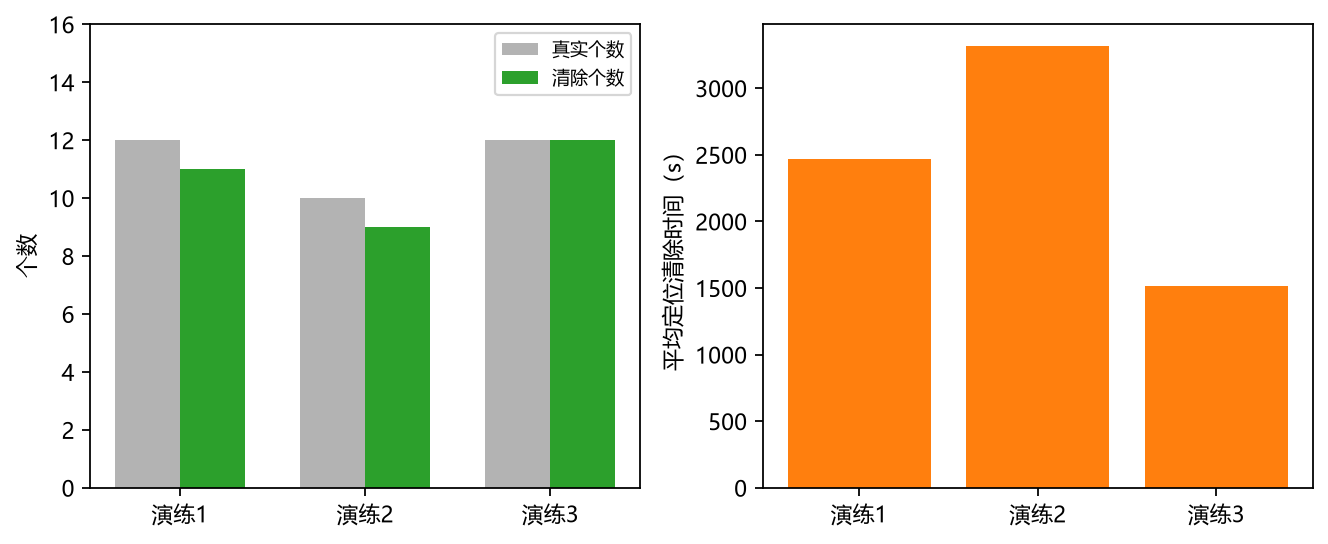
\includegraphics[width=0.98\textwidth]{figures/q4_rehearsal_bars.png}
\caption{问题四窗口三次演练：真实个数与清除个数；右幅为平均定位清除时间。该组对应$900/2100$ m同辐条网，不是三角格网加保扇形。}
\label{fig:q4reh}
\end{figure}

问题四正式测试格式与问题三相同，见表\ref{tab:official4}。定向朝向由模拟器生成，正文不假设朝向分布。表\ref{tab:q4reh}、表\ref{tab:q4full}与表\ref{tab:q4m2}的演练行不得抄入该表。

\begin{table}[htbp]
\centering
\caption{问题四正式测试结果（格式同题目表1）}
\label{tab:official4}
\begin{tabular}{lcccc}
\toprule
测试 & 案例编码 & 清除干扰源个数 & 平均定位清除时间 & 程序运行时间 \\
\midrule
测试1 & --- & --- & --- & --- \\
测试2 & --- & --- & --- & --- \\
测试3 & --- & --- & --- & --- \\
\bottomrule
\end{tabular}
\end{table}

\FloatBarrier
\subsection{诊断}

格网发现引理在$R_{\mathrm{eff}}\ge 1000$ m且瓣为闭$180^\circ$时给出$\forall G\forall u$必被某一格点听到，不保证一次测向就把$R_{\mathrm{sec}}$压到20 m。最近剩余与保扇形$(r,t)$列表是时间启发式；证书动作是走完剩余格点、以及$R_{\mathrm{sec}}\le 20$ m的圆心清除。侧向$S+tv$只在$v\perp H$时对一切$t$留瓣；沿测得示向度越过源的半平面翻转只在精确方位下成立。光学方格只在$R_{\mathrm{sec}}\le 80$ m时作为清除证书；更大的定位区上圆心强制\texttt{/clear}不是覆盖证书。修订问题三的有限动作全清证明依赖全向源假设，不能移用于本节的定向瓣；现实程序期限、测试窗口与技术异常仍可能造成未完成。混编覆盖循环同样在这些情形返回，格网引理不删除该残差。1536点网格全部可听只是核对。表\ref{tab:q4reh}前两次分别清除$11/12$与$9/10$，对应的是半径$900$ m与$2100$ m的同辐条网以及交付点$(800,700)$ m长跨步，不是$\rho=s/\sqrt{3}<500$ m的有限格点引理在同一策略上的经验剩余。表\ref{tab:q4full}三次全部清除，只说明边长$850$ m的$37$点格网加保扇形在这三个独立案例上把示向度收进了清除圆；发现层的覆盖结论仍由闭式界给出。表\ref{tab:q4m2}是方法二的时间层展示：合并不配对均值318.1 s/已清，三次中有两次未全部清除，因而不是发现证书，也不能回写成$\forall G\forall u$必听到。频道优先当前测向机、命中即追逐，这两条规则在混编情形同样节省换台。沿示向度的长跨步会把第二站送出$180^\circ$瓣，不能作为定向源的默认第二站。演练结束时模拟器返回总数，因而比例可算；正式测试只报告清除个数与平均时间。

\section{灵敏度分析}

\subsection{横向偏移}

灵敏度只扰动能够移动决策的量。由表\ref{tab:q2sens}可知，固定轴向距离1100 m时，横向偏移从200 m增到800 m，中位直径由93.12 m降到58.03 m，下降35.09 m，决策取较大$t$。$t$继续增到1000 m时，1000 m可听比例降到约0.07，直径中位数回升到60.29 m，故候选带把$|t|$上截在约845 m。如图\ref{fig:sens}所示，该剖面是$(r,t)=(1100,800)$ m，与交付点$(800,700)$ m不是同一组坐标。交付点$|t|=700$ m由$r=800$ m处轴上$\psi\ge 45^\circ$覆盖给出，即$|t|\ge 1500-800$；它不是把网格分位$690.9$ m圆整，也不是把$(1100,800)$ m剖面当作取700 m的依据。网格分位点远轴$\psi\approx 44.63^\circ$，不覆盖该引理。

\subsection{楔半角}

楔半角扫描取剖面$(r,t)=(1100,500)$ m。半角从$0.5^\circ$变到$1^\circ$，一次清除从1变到0；再增到$1.5^\circ$，中位直径升到92.65 m。如图\ref{fig:errsweep}所示，绿虚线在$1^\circ$处由1翻转到0，对应的是该$(1100,500)$ m剖面。网格分位点$(r,t)=(800,690.9)$ m的一次清除比例为$\eta_1=0.21$，中位直径为48.27 m，与上述翻转不是同一组$(r,t)$；交付点是$(800,700)$ m。题设$1^\circ$在$(1100,500)$ m处恰好卡在一次清除的边界上。

\subsection{三角格间距}

问题四的发现证书随格点间距$s$翻转。覆盖半径$\rho=s/\sqrt{3}$，合格平移量存在当且仅当$\rho<500$ m，即$s<500\sqrt{3}\approx 866.03$ m。如图\ref{fig:ablation}所示，$\rho$随$s$线性上升，在$s=850$ m处低于500 m，在$s=900$ m处高于500 m；等号$s=500\sqrt{3}$使$\rho=500$，开距离盘条件不成立。由表\ref{tab:ablation}可知，$s=850$ m时$\rho\approx 490.75$ m，存在合格平移量，$a+\rho\approx 990.75$ m；同一截断规则下有限格点为37个。$s=900$ m时$\rho\approx 519.62$ m，合格平移量为0。$s=700$ m时覆盖半径更小，但有限格点增至55个，移动项增加。交付间距因此取850 m：它严格小于上界，又不必把网加密到700 m。该扫描不改换模型类，只扰动能够翻转“是否存在合格$a$”的量。

\begin{figure}[htbp]
\centering
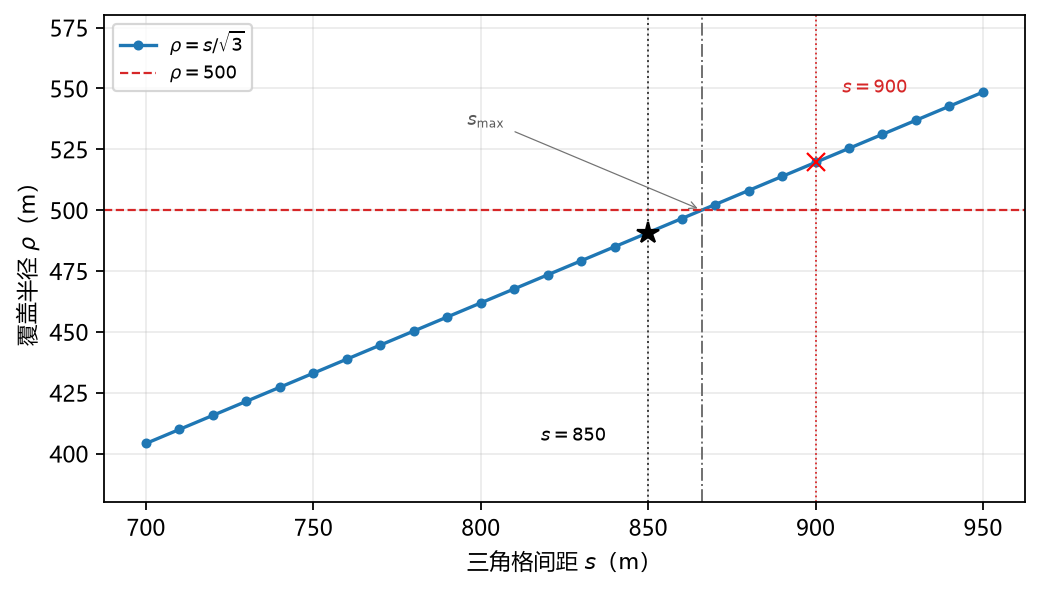
\includegraphics[width=0.82\textwidth]{figures/q4_ring_ablation.png}
\caption{三角格覆盖半径随间距的变化。水平虚线为$\rho=500$ m；星号为交付间距$s=850$ m，叉号为不合格间距$s=900$ m。}
\label{fig:ablation}
\end{figure}

\begin{table}[htbp]
\centering
\caption{三角格间距扫描：覆盖半径与合格平移量}
\label{tab:ablation}
\begin{tabular}{rrrrr}
\toprule
$s$ / m & $\rho$ / m & 存在$a$ & $a+\rho$ / m & 格点数 \\
\midrule
700 & 404.15 & 1 & 904.15 & 55 \\
800 & 461.88 & 1 & 961.88 & 37 \\
850 & 490.75 & 1 & 990.75 & 37 \\
866.03 & 500.00 & 0 & 1000.00 & 37 \\
900 & 519.62 & 0 & 1019.62 & 37 \\
950 & 548.48 & 0 & 1048.48 & 31 \\
\bottomrule
\end{tabular}
\end{table}

\subsection{场地裁剪}

问题一的场地裁剪把对径圆覆盖率从1降到0.955，说明直径圆的覆盖结论必须声明是否与场地相交。问题三把侦听半径取1000 m而不是1500 m，覆盖率为1，决策偏保守但可执行。

这些扫描都不改换模型类：楔形交、直径、侦听覆盖与追逐判定保持不变。侦听点加密会增加移动项，正文只报告满足覆盖约束的网。

\section{模型评价}

\subsection{优点}

本文把示向度误差写成凸楔形，把交会写成半平面裁剪，把清除写成最小包围圆与清除半径的比较，机理可解释、方程可核验。问题一明确给出对径圆覆盖不是恒真，并用等边三角形与三站六边形展示失败模式。问题二用轴上$\psi\ge 45^\circ$覆盖给出可复现的第二站，交角中位数接近直角。问题三将9点覆盖、严格保守剪枝与有界收缩结合，在题设模型和有效接口响应条件下给出有限动作全清定理，动作上界为294；访问顺序用开放TSP与最近服务入口优化。$A_{\max}=900$是算法自设闸，不是题面常数。问题四在同一几何口径上改用边长850 m的三角格网，把定向发现写成覆盖半径$\rho<500$ m的闭式证书，并用保扇形第二站与光学方格完成局部化。原包列出的定量结论包括：正交例直径34.92 m且对径圆覆盖；网格分位点直径中位数48.27 m、一次清除$15/70$；交付点横向700 m覆盖轴上$\psi\ge 45^\circ$；9点覆盖半径956.05 m；37点格网覆盖半径490.75 m，平移量和990.75 m，光学方格外接半径17.68 m。论文体例遵循竞赛格式规范\cite{format}。

\subsection{不足}

第一，有效接收半径未知，侦听网按下限设计，真实半径更大时网偏密、移动偏多。第二，题设$1^\circ$下两站一次清除比例$\eta_1=15/70=0.21$，修订Q3用保守距离上界收缩清除，仍可能增加移动量，未证明时间最优。第三，格网发现引理保证听到，不保证一次测向就把$R_{\mathrm{sec}}$压到20 m；光学方格只在$R_{\mathrm{sec}}\le 80$ m时是清除证书。窗口三次中前两次分别清除$11/12$与$9/10$，来自$900/2100$ m网与$(800,700)$ m追逐，不能当作$\rho=s/\sqrt{3}<500$ m有限格点引理的经验剩余；本文实现在随后三个独立案例上全部清除，只说明这三个案例收到了清除圆。第四，侧向留瓣当且仅当$v\perp H$，保扇形$(r,t)$表是时间启发式。第五，演练比例以返回的总数为分母，正式测试按题目表1只报告清除个数与平均时间，二者不可混填。修订Q3给出了有限动作证明，但该证明不保证网络和现实窗口始终可用；旧演练数据不能验证新代码的实测速度，修订版官方演练及三次正式日志仍待补齐。

\subsection{推广}

把楔形半角从仪器标定读入后，同一套裁剪与直径算法可用于其它测向平台。第二站的轴上覆盖点可以按清除半径重算，不一定钉在800 m与700 m；全向源应先完成有限覆盖，再用有界收缩或其它经认证的局部化方法清除，定向源则应继续使用短沿迹加侧向，而不是把全向交付点直接移植。三角格间距可按实际$R_{\mathrm{eff}}$重算，使$\rho<R_{\mathrm{eff}}/2$。若允许第二只机器狗，正交基线可以由两台同时占用，虚拟时间中的移动项会下降。无论推广到哪一步，示向度都不能退回成无误差射线，正式测试次数也不能用演练行顶替。

AI工具使用情况见同目录文件《AI工具使用详情》。

\begin{thebibliography}{99}
\bibitem{stansfield1947} Stansfield R G. Statistical theory of d.f. fixing[J]. Journal of the Institution of Electrical Engineers, Part IIIA: Radiocommunication, 1947, 94(15): 762-770.
\bibitem{torrieri1984} Torrieri D J. Statistical theory of passive location systems[J]. IEEE Transactions on Aerospace and Electronic Systems, 1984, 20(2): 183-198.
\bibitem{nardone1984} Nardone S C, Lindgren A G, Gong K F. Fundamental properties and performance of conventional bearings-only target motion analysis[J]. IEEE Transactions on Automatic Control, 1984, 29(9): 775-787.
\bibitem{foy1976} Foy W H. Position-location solutions by Taylor-series estimation[J]. IEEE Transactions on Aerospace and Electronic Systems, 1976, 12(2): 187-194.
\bibitem{jung1901} Jung H. \"{U}ber die kleinste Kugel, die eine r\"{a}umliche Figur einschlie{\ss}t[J]. Journal f\"{u}r die reine und angewandte Mathematik, 1901, 123: 241-257.
\bibitem{welzl1991} Welzl E. Smallest enclosing disks (balls and ellipsoids)[C]//Maurer H. New Results and New Trends in Computer Science. Lecture Notes in Computer Science, vol. 555. Berlin: Springer, 1991: 359-370.
\bibitem{sutherland1974} Sutherland I E, Hodgman G W. Reentrant polygon clipping[J]. Communications of the ACM, 1974, 17(1): 32-42.
\bibitem{toussaint1983} Toussaint G T. Solving geometric problems with the rotating calipers[C]//Proceedings of IEEE MELECON. 1983.
\bibitem{dogancay2005} Dogancay K. Bearings-only target localization using total least squares[J]. Signal Processing, 2005, 85(9): 1695-1710.
\bibitem{bishop2010} Bishop A N, Fidan B, Anderson B D O, Dogancay K, Pathirana P N. Optimality analysis of sensor-target geometries in passive localization[J]. Automatica, 2010, 46(3): 479-492.
\bibitem{clarke1964} Clarke G, Wright J W. Scheduling of vehicles from a central depot to a number of delivery points[J]. Operations Research, 1964, 12(4): 568-581.
\bibitem{format} 全国大学生数学建模竞赛组委会. 全国大学生数学建模竞赛论文格式规范[S].
\end{thebibliography}

\appendix
\section{支撑材料}

\subsection{问题一顶点与Monte Carlo样本}

表\ref{tab:q1vert}的四个顶点复述如下，供独立核验直径34.92 m。Monte Carlo请求400个样本，种子2026，全部有界，382个对径圆覆盖，覆盖率0.955；正文直方图与散点使用这400行，不是子样本。

\begin{table}[htbp]
\centering
\caption{正交交会例顶点（与表\ref{tab:q1vert}相同）}
\label{tab:q1vertapp}
\begin{tabular}{crr}
\toprule
编号 & $x$ / m & $y$ / m \\
\midrule
1 & 500.000 & 517.765 \\
2 & 482.550 & 499.695 \\
3 & 500.000 & 482.844 \\
4 & 517.450 & 499.695 \\
\bottomrule
\end{tabular}
\end{table}

\begin{table}[htbp]
\centering
\caption{问题一有界样本容量}
\label{tab:q1mcmeta}
\begin{tabular}{lr}
\toprule
量 & 取值 \\
\midrule
种子 & 2026 \\
请求样本数 & 400 \\
有界样本数 & 400 \\
对径圆覆盖个数 & 382 \\
覆盖率 & 0.955 \\
CSV行数 & 400 \\
\bottomrule
\end{tabular}
\end{table}


\subsection{侦听点坐标}

问题三点位见表\ref{tab:q3xy}。问题四侦听网为边长850 m的三角格点截断到$\mathbb{D}(0,1800+500+\rho)$，共37点，见表\ref{tab:q4visit}。下一站取最近剩余点，该表是点位清单而不是固定走环。

{\scriptsize
\begin{longtable}{crrl}
\caption{问题四三角格网点位清单（下一站取最近剩余点）}
\label{tab:q4visit}\\
\toprule
编号 & $x$ / m & $y$ / m & 角色 \\
\midrule
\endfirsthead
\toprule
编号 & $x$ / m & $y$ / m & 角色 \\
\midrule
\endhead
1 & $-2550.0$ & 0.0 & 三角格点 \\
2 & $-2125.0$ & $-736.1$ & 三角格点 \\
3 & $-2125.0$ & 736.1 & 三角格点 \\
4 & $-1700.0$ & $-1472.2$ & 三角格点 \\
5 & $-1700.0$ & 0.0 & 三角格点 \\
6 & $-1700.0$ & 1472.2 & 三角格点 \\
7 & $-1275.0$ & $-2208.4$ & 三角格点 \\
8 & $-1275.0$ & $-736.1$ & 三角格点 \\
9 & $-1275.0$ & 736.1 & 三角格点 \\
10 & $-1275.0$ & 2208.4 & 三角格点 \\
11 & $-850.0$ & $-1472.2$ & 三角格点 \\
12 & $-850.0$ & 0.0 & 三角格点 \\
13 & $-850.0$ & 1472.2 & 三角格点 \\
14 & $-425.0$ & $-2208.4$ & 三角格点 \\
15 & $-425.0$ & $-736.1$ & 三角格点 \\
16 & $-425.0$ & 736.1 & 三角格点 \\
17 & $-425.0$ & 2208.4 & 三角格点 \\
18 & 0.0 & $-1472.2$ & 三角格点 \\
19 & 0.0 & 0.0 & 原点 \\
20 & 0.0 & 1472.2 & 三角格点 \\
21 & 425.0 & $-2208.4$ & 三角格点 \\
22 & 425.0 & $-736.1$ & 三角格点 \\
23 & 425.0 & 736.1 & 三角格点 \\
24 & 425.0 & 2208.4 & 三角格点 \\
25 & 850.0 & $-1472.2$ & 三角格点 \\
26 & 850.0 & 0.0 & 三角格点 \\
27 & 850.0 & 1472.2 & 三角格点 \\
28 & 1275.0 & $-2208.4$ & 三角格点 \\
29 & 1275.0 & $-736.1$ & 三角格点 \\
30 & 1275.0 & 736.1 & 三角格点 \\
31 & 1275.0 & 2208.4 & 三角格点 \\
32 & 1700.0 & $-1472.2$ & 三角格点 \\
33 & 1700.0 & 0.0 & 三角格点 \\
34 & 1700.0 & 1472.2 & 三角格点 \\
35 & 2125.0 & $-736.1$ & 三角格点 \\
36 & 2125.0 & 736.1 & 三角格点 \\
37 & 2550.0 & 0.0 & 三角格点 \\
\bottomrule
\end{longtable}
}

\subsection{实现注记}

机器狗标识取队号，场地标识取默认值。串行等待上一次返回后再发下一次请求。附录所列源文件给出楔形交、直径、侦听网与追逐的可运行实现。问题三表\ref{tab:q3reh}保留旧启发式的三次历史演练；修订实现位于\texttt{code/q3/searcher.py}，新验证记录在\texttt{code/q3/offline\_results.json}。问题四表\ref{tab:q4full}对应边长$850$ m的三角格网加保扇形；表\ref{tab:q4reh}对应窗口中$900/2100$ m同辐条网与交付点$(800,700)$ m，两组都不是正式测试，也不得混填。

{\small
\begin{tabular}{ll}
\toprule
路径 & 功能 \\
\midrule
\texttt{wedge\_quad/experiment.py} & 楔形交、直径与第二站比较 \\
\texttt{wedge\_quad/geom.py} & 半平面裁剪与最小包围圆 \\
\texttt{wedge\_quad/sensitivity.py} & 横向偏移与半角扫描 \\
\texttt{bearing\_chase/experiment.py} & 侦听覆盖 \\
\texttt{bearing\_chase/searcher.py} & 侦听网与楔形追逐 \\
\texttt{bearing\_chase/geom.py} & 追逐几何例程 \\
\texttt{paper/plot\_paper.py} & 展示用图与表 \\
\bottomrule
\end{tabular}
}

\end{document}
